
\chapter[Redundancy under Discussion]{Redundancy under Discussion\footnotemark}\label{chap:redundancy}
\footnotetext{This Chapter constitutes a longer and hopefully more readable adaptation of \citettoappear{HenotMortier2024b}. I would like to thank the audience and reviewers of SuB29 and of the 2024 BerlinBrnoVienna Workshop, in particular Itai Bassi, for relevant questions, datapoints and suggestions regarding earlier iterations of this project.}

This chapter presents novel data derived from the logical form $p\vee p \vee q$, \textit{via} the \textit{or}-to-\textit{if} tautology and core properties of disjunction (commutativity, associativity). The sentences at stake exhibit differing degrees of pragmatic oddness, which is shown to represent a challenge for existing theories of oddness. Building on the machinery defined in Chapter \ref{chap:accommodating-quds}, we propose a solution the this paradigm in term of QuD-driven \textsc{Redundancy}. More broadly, this Chapter motivates the use of implicit QuDs, which are semantically richer than the Logical Forms they are derived from, to evaluate pragmatic oddness.


\section{A problematic dataset}

The disjunctive sentences in (\ref{ex4:double-disjunctions}), which are logically related to each other \textit{via} applications of $\vee$-commutativity and $\vee$-associativity, appear sharply infelicitous.\footnote{More variants could be derived, for instance $q\vee(p\vee p)$. Here, we focus on the less obvious variants where two instances of $p$ do not directly combine together.} Such sentences can be seen as pragmatically odd due to them being contextually equivalent to their complex disjunct, whether it is $p\vee q$, or $q \vee p$ \citep{Katzir2014}.

\begin{exe}
	\ex \textit{Context: Jo is supposed to attend Sinn und Bedeutung in Italy, but is also busy writing his MIT dissertation. Jo's friend are at the conference and wonder if he is around.}\label{ex4:double-disjunctions}
	\begin{xlist}
		\ex[\#] {Either Jo is at SuB, or else he is at SuB or in Cambridge.\hfill $\p\vee (\p \vee \q)$}\label{ex4:pv(pvq)}
		\ex[\#] {Either Jo is at SuB, or else he is in Cambridge or at SuB.\hfill $\p\vee (\q \vee \p)$}\label{ex4:pv(qvp)}
		\ex[\#] {Either Jo is at SuB or in Cambridge, or else he is at SuB.\hfill $(\p \vee \q) \vee \p$}\label{ex4:(pvq)vp}
		\ex[\#] {Either Jo is in Cambridge or at SuB, or else he is at SuB.\hfill $(\q \vee \p) \vee \p$}\label{ex4:(qvp)vp}
	\end{xlist}
\end{exe} 

(\ref{ex4:pv(pvq)-variants}-\ref{ex4:(qvp)vp-variants}) show variants of (\ref{ex4:pv(pvq)}-\ref{ex4:(qvp)vp}) obtained \textit{via} the \textit{or}-to-\textit{if} tautology. In each pair of sentences, the a. instances are derived by modifying the outer disjunction, while the the b. instances are derived by modifying the inner disjunction.\footnote{One could also apply the \textit{or}-to-\textit{if} tautology to \textit{both} the inner and the outer disjunction in the sentences in (\ref{ex4:double-disjunctions}). Nested conditionals however, are hard to judge. We will briefly cover them in Section \ref{sec4:double-or-if}.}. Note that we do not intend to commit to a material analysis of the conditionals featured in these examples. Throughout this Chapter, $\rightarrow$ will be used as a mere shorthand for \textit{if... then...}, i.e. will not imply that the conditionals under consideration are necessarily material.\\


\begin{exe}
	\ex Derived from (\ref{ex4:pv(pvq)}):
	\begin{xlist}
		\ex[\#] {If Jo is not at SuB then he is at SuB or in Cambridge.\\ $\neg \p \rightarrow (\p \vee \q)$}\label{ex4:npt(pvq)}
		\ex[] {Either Jo is at SuB or if he is not at SuB then he is in Cambridge.\\ $\p \vee (\neg \p \rightarrow \q)$}\label{ex4:pv(nptq)}
	\end{xlist}\label{ex4:pv(pvq)-variants}
	\ex Derived from (\ref{ex4:pv(qvp)}):
	\begin{xlist}
		\ex[\#] {If Jo is not at SuB then he is in Cambridge or at SuB.\\ $\neg \p \rightarrow (\q \vee \p)$}\label{ex4:npt(qvp)}
		\ex[\#] {Either Jo is at SuB or if he is not in Cambridge then he is at SuB.\\ $\p \vee (\neg \q \rightarrow \p)$}\label{ex4:pv(nqtp)}
	\end{xlist}\label{ex4:pv(qvp)-variants}
	\ex Derived from (\ref{ex4:(pvq)vp}):
	\begin{xlist}
		\ex[\#] {If it's not true that Jo is at SuB or in Cambridge, then he is at SuB.\\ $\neg (\p \vee \q) \rightarrow \p$}\label{ex4:n(pvq)tp}
		\ex[?] {Either Jo is in Cambridge if not at SuB, or he is at SuB.\\ $(\neg \p \rightarrow \q) \vee \p$}\label{ex4:(nptq)vp}
	\end{xlist}\label{ex4:(pvq)vp-variants}
	\ex Derived from (\ref{ex4:(qvp)vp}):
	\begin{xlist}
		\ex[\#] {If it's not true that Jo is in Cambridge or at SuB, then he is at SuB.\\ $\neg (\q \vee \p) \rightarrow \p$}\label{ex4:n(qvp)tp}
		\ex[\#] {Either Jo is at SuB if not in Cambridge, or he is at SuB.\\ $(\neg \q \rightarrow \p) \vee \p$}\label{ex4:(nqtp)vp}
	\end{xlist}\label{ex4:(qvp)vp-variants}
\end{exe} 

Surprisingly, these variants exhibit different degrees of oddness: (\ref{ex4:pv(nptq)}) and (\ref{ex4:(nptq)vp}) escape infelicity, while the other variants do not.\footnote{(\ref{ex4:(nptq)vp}) sounds more degraded than (\ref{ex4:pv(nptq)}) however. We come back to this contrast in Section \ref{sec4:ordering}.} This is unexpected given that all the sentences in (\ref{ex4:pv(pvq)-variants}-\ref{ex4:(qvp)vp-variants}) have same logical structure as the infelicitous sentences in (\ref{ex4:pv(pvq)}-\ref{ex4:(qvp)vp}), assuming implications are material (we will see that, in fact, issues remain when conditionals are \textit{not} treated as material). Particularly puzzling is the existence of a contrast \textit{between} the different b. examples in (\ref{ex4:pv(pvq)-variants}-\ref{ex4:(qvp)vp-variants}), which are derived from (\ref{ex4:pv(pvq)}-\ref{ex4:(qvp)vp}) using the \textit{same} transformation.


The descriptive generalization seems to be the following: the sentences in (\ref{ex4:pv(pvq)-variants}-\ref{ex4:(qvp)vp-variants}) that retain an outer disjunction, and whose complex (conditional) disjunct has the negation of their simple disjunct as antecedent, are rescued.



In this Chapter, we propose that this descriptive generalization follows from the idea that oddness arises when sentences cannot evoke any well-formed implicit QuD, as defined in Chapter \ref{chap:accommodating-quds}. The crucial point proposed in Chapter \ref{chap:accommodating-quds}  that we will exploit here, is that disjunctions and conditionals give rise to different implicit QuDs. This model of accommodated QuDs will lead us to introduce a new notion of redundancy, \textsc{Q-Non-Redundancy}, that applies to pairs formed by LFs and accommodated QuDs -- instead of just LFs. Under this view, sentences like (\ref{ex4:pv(nptq)}) and (\ref{ex4:(nptq)vp}) whose re-occurring material ($p$), each time plays different roles w.r.t. the QuD (typically, as a disjunct, or as a conditional ``restrictor''), can escape \textsc{Q-Non-Redundancy}.\\


Assuming that the sole application $\vee$-commutativity does not affect oddness (generally in line with the data presented here), we now focus on sentences (\ref{ex4:pv(pvq)}), (\ref{ex4:npt(pvq)}), (\ref{ex4:pv(nptq)}), (\ref{ex4:pv(nqtp)}), and (\ref{ex4:n(pvq)tp}), repeated in that order in (\ref{ex4:target-sentences}).
\begin{exe}
	\ex \label{ex4:target-sentences}
	\begin{xlist}
		\ex[\#] {Either Jo is at SuB, or else he is at SuB or in Cambridge.\\ \hfill $\p\vee (\p \vee \q)$}\label{ex4:pv(pvq)-repeated}
		\ex[\#] {If Jo is not at SuB then he is at SuB or in Cambridge.\\ \hfill $\neg \p \rightarrow (\p \vee \q)$}\label{ex4:npt(pvq)-repeated}
		\ex[] {Either Jo is at SuB or if he is not at SuB then he is in Cambridge.\\ \hfill $\p \vee (\neg \p \rightarrow \q)$}\label{ex4:pv(nptq)-repeated}
		\ex[\#] {Either Jo is at SuB or if he is not in Cambridge then he is at SuB.\\ \hfill $\p \vee (\neg \q \rightarrow \p)$}\label{ex4:pv(nqtp)-repeated}
		\ex[\#] {If it's not true that Jo is at SuB or in Cambridge, then he is at SuB.\\ \hfill $\neg (\p \vee \q) \rightarrow \p$}\label{ex4:n(pvq)tp-repeated}
	\end{xlist}
\end{exe}


The rest of this Chapter is structured as follows. The next Section reviews why some of the sentences in (\ref{ex4:target-sentences}) are problematic for existing accounts of oddness. Section \ref{sec4:my-account} briefly summarizes the model of implicit QuDs laid out in Chapter \ref{chap:accommodating-quds} and shows how it derives different QuDs for the disjunctions and conditionals at stake. Section \ref{sec4:Q-Non-Redundancy} defines a new \textsc{Non-Redundancy} constraint targeting pairs formed by LFs and their accommodated QuD, and shows how this constraint captures the contrasts in (\ref{ex4:target-sentences}). Section \ref{sec4:stock} compares the constraint to those posited by similar earlier accounts and further connects it to \citeauthor{Grice1975}'s  \textsc{Maxim of Manner}.
Section \ref{sec4:exploration} discusses a few additional datapoints related to (\ref{ex4:target-sentences}), and Section \ref{sec4:conclusion} concludes the Chapter.

\section{Previous accounts of oddness, and their shortcomings}\label{sec4:previous-accounts}

In this section we present four existing accounts of oddness: \textsc{Global Non-Redundancy}, \textsc{Local Non-Redundancy}, \textsc{Super-Redundancy}, and \textsc{Non-Triviality} (see \citenp{Marty2022} for a more complete overview of these principles). The first three accounts are based on the notion of redundancy, which can be traced back to Grice's Maxim of Manner (submaxim of \textsc{Brevity}, \citenp{Grice1975}). The last account exploits the notion of triviality \citep{Stalnaker1974}. We show that all accounts straightforwardly capture the double disjunction case (\ref{ex4:pv(pvq)-repeated}). However, the first three accounts fall short in explaining the contrast between the felicitous (\ref{ex4:pv(nptq)-repeated}) and the infelicitous (\ref{ex4:npt(pvq)-repeated}), (\ref{ex4:pv(nqtp)-repeated}), and (\ref{ex4:n(pvq)tp-repeated}). The last account on the other hand, \textit{can} capture the pattern in (\ref{ex4:target-sentences}), but at the cost of mispredicting the classic pattern of so-called Hurford Disjunctions \citep{Hurford1974}.

\subsection{Global Non-Redundancy}

\textsc{Redundancy}-based accounts of oddness based on Grice's submaxim of \textsc{Brevity}, which is part of the maxim of \textsc{Manner}, defined in (\ref{ex4:manner}).

\begin{exe}
	\ex {\textsc{\textbf{Maxim of Manner}} \citep{Grice1975}. Be clear, meaning:
		\begin{enumerate}
			\item Avoid obscurity of expression -- i.e., avoid language that is difficult to understand;
			\item Avoid ambiguity -- i.e., avoid language that can be interpreted in multiple ways;
			\item Be brief -- i.e., avoid unnecessary verbosity;
			\item Be orderly -- i.e., provide information in an order that makes sense, and makes it easy for the recipient to process it.
		\end{enumerate}}\label{ex4:manner}
\end{exe}

According to this view, sentences that feature unnecessary verbosity should be deemed odd. This is cashed out in (\ref{ex4:global-non-redundancy}), which states that, if two sentences are contextually equivalent, then the simpler one should be preferred, and the more complex one should be deviant. Simplicity is understood as structural, following \citet{Katzir2007} -- see (\ref{ex4:structural-complexity}). We dub the principle in (\ref{ex4:global-non-redundancy}) \textsc{Global Non-Redundancy}, because contextual equivalence and simplicity are evaluated at the level of the entire sentence, and not locally.\footnote{A local variant of this principle will be investigated in the next Section.}

\begin{exe}
	\ex {\textsc{\textbf{Global Non-Redundancy}} \citep{Meyer2013,Mayr2016}. A sentence $S$ cannot be used in context $c$ if there is a sentence $S'$ s.t. $S'$ is a simplification of $S$ and $S' \equiv_c S$.}\label{ex4:global-non-redundancy}
	\ex {\textsc{\textbf{Structural simplicity}} \citep{Katzir2007}. $S'$ is a simplification of $S$ if $S'$ can be derived from $S$ by replacing nodes in $S$ with their subconstituents.}\label{ex4:structural-complexity}
\end{exe}

(\ref{ex4:global-non-redundancy}) predicts the double disjunction (\ref{ex4:pv(pvq)-repeated}) to be deviant, because it is contextually equivalent to its complex disjunct ($p\vee q$). The same can be said of all other variants in (\ref{ex4:target-sentences}), see (\ref{ex4:gnr-material}). In brief, (\ref{ex4:global-non-redundancy}) does not derive the expected contrast between the felicitous (\ref{ex4:pv(nptq)-repeated}) on the one hand, and the infelicitous (\ref{ex4:pv(pvq)-repeated}), (\ref{ex4:npt(pvq)-repeated}), (\ref{ex4:pv(nqtp)-repeated}), and (\ref{ex4:n(pvq)tp-repeated}), on the other.

\begin{exe}
	\ex Applying \textsc{Global Non-Redundancy} (abbreviated GNR) to the sentences in (\ref{ex4:target-sentences}), under the assumption conditionals are material. Underlined constituents are the ones the entire expressions end up being contextually equivalent to. \label{ex4:gnr-material}
	\begin{xlist}
		\ex {(\ref{ex4:pv(pvq)-repeated}): $\p \vee (\underline{\p \vee \q}) \equiv \p \vee \q$ \hfill GNR \xmark}\label{ex4:pv(pvq)-gnr-material}
		\ex {(\ref{ex4:npt(pvq)-repeated}): $\neg \p \rightarrow (\underline{\p \vee \q}) \equiv \p \vee (\p \vee \q) \equiv \p \vee \q$ \hfill GNR \xmark}\label{ex4:npt(pvq)-gnr-material}
		\ex {(\ref{ex4:pv(nptq)-repeated}): $\p \vee (\underline{\neg \p \rightarrow \q}) \equiv \p \vee (\p \vee \q) \equiv \p \vee \q \equiv \neg\p \rightarrow \q$\hfill GNR \xmark}\label{ex4:pv(nptq)-gnr-material}
		\ex {(\ref{ex4:pv(nqtp)-repeated}): $\p \vee (\underline{\neg \q \rightarrow \p}) \equiv \p \vee (\q \vee\p) \equiv \p \vee \q \equiv \neg \q \rightarrow \p $ \hfill GNR \xmark}\label{ex4:pv(nqtp)-gnr-material}
		\ex {(\ref{ex4:n(pvq)tp-repeated}): $\neg(\underline{\p \vee \q}) \rightarrow \p \equiv (\p \vee \q) \vee \p \equiv \p \vee \q $ \hfill GNR \xmark}\label{ex4:n(pvq)tp-gnr-material}
	\end{xlist}
\end{exe}

Assuming conditionals a non-material does not help. Under this assumption, the prediction for the double disjunction (\ref{ex4:pv(pvq)-repeated}) does not change, but those for the ``conditional'' variants (\ref{ex4:npt(pvq)-repeated}-\ref{ex4:n(pvq)tp-repeated}), may change. Since a non-material conditional is never contextually equivalent to its antecedent or consequent, regardless of what they denote, one can focus on disjunct simplifications of (\ref{ex4:npt(pvq)-repeated}-\ref{ex4:n(pvq)tp-repeated}) when evaluating (\ref{ex4:global-non-redundancy}). Moreover, one can focus on simplifications retaining an occurrence of $q$, since these are the only ones which may turn out equivalent to the entire expressions (which involve $q$). Such simplifications are collected in (\ref{ex4:disjunct-simplifications}).

\begin{exe}
	\ex Computing potentially equivalent simplifications of (\ref{ex4:npt(pvq)-repeated}-\ref{ex4:n(pvq)tp-repeated}) \label{ex4:disjunct-simplifications}
	\begin{xlist}
		\ex {(\ref{ex4:npt(pvq)-repeated}): $\neg \p \rightarrow (\cancel{\p \vee} \q)= \neg \p \rightarrow \q$}\label{ex4:npt(pvq)-simp}
		\ex {(\ref{ex4:pv(nptq)-repeated}): $\cancel{\p \vee} (\neg \p \rightarrow \q) = \neg \p \rightarrow \q$}\label{ex4:pv(nptq)-simp}
		\ex {(\ref{ex4:pv(nqtp)-repeated}): $\cancel{\p \vee} (\neg \q \rightarrow \p) = \neg \q \rightarrow \p$}\label{ex4:pv(nqtp)-simp}
		\ex {(\ref{ex4:n(pvq)tp-repeated}): $\neg(\cancel{\p \vee} \q) \rightarrow \p = \neg \q \rightarrow \p$}\label{ex4:n(pvq)tp-simp}
	\end{xlist}
\end{exe}

One can then evaluate the contextual equivalence between the candidate simplifications in (\ref{ex4:disjunct-simplifications}), and the entire expressions in (\ref{ex4:npt(pvq)-repeated}-\ref{ex4:n(pvq)tp-repeated}). Assuming conditionals are strict, we find that (\ref{ex4:npt(pvq)-repeated}) and (\ref{ex4:n(pvq)tp-repeated}) are equivalent to their simplifications in (\ref{ex4:npt(pvq)-simp}) and (\ref{ex4:n(pvq)tp-simp}), respectively, so should be deemed deviant, in line with intuitions. Both (\ref{ex4:pv(nptq)-repeated}) and (\ref{ex4:pv(nqtp)-repeated}) however, are logically independent from their only reasonable simplifications (\ref{ex4:pv(nptq)-simp}) and (\ref{ex4:pv(nqtp)-simp}), and therefore, should both be felicitous. This is a good prediction for (\ref{ex4:pv(nptq)-repeated}), but a bad prediction for (\ref{ex4:pv(nqtp)-simp}). In brief, assuming conditionals are strict, improves the ``fit'' of principle (\ref{ex4:global-non-redundancy}), but still, fails at capturing the entire picture.

\begin{exe}
	\ex\label{ex4:gnr-strict} Applying \textsc{Global Non-Redundancy} (abbreviated GNR) to (\ref{ex4:npt(pvq)-repeated}-\ref{ex4:n(pvq)tp-repeated}), under the assumption conditionals are strict, and considering the candidate simplification computed in (\ref{ex4:disjunct-simplifications}). 
	\begin{xlist}
			\ex {(\ref{ex4:npt(pvq)-repeated}) $\equiv$ every $\neg \p$-world is a \p- or a \q-world\\
				\phantom{(\ref{ex4:npt(pvq)-repeated}) }$\equiv$ every $\neg \p$-world is a \q-world\\
				\phantom{(\ref{ex4:npt(pvq)-repeated}) }$\equiv$ (\ref{ex4:npt(pvq)-simp}) \hfill GNR \xmark}
			\ex {(\ref{ex4:pv(nptq)-repeated}) $\equiv$ \p{} or every $\neg$\p-world is a \q-world\\
				\phantom{(\ref{ex4:pv(nptq)-repeated}) }$\not\equiv$ every $\neg$\p-world is a \q-world $\equiv$ (\ref{ex4:pv(nptq)-simp}) \hfill GNR \cmark}
			\ex {(\ref{ex4:pv(nqtp)-repeated}) $\equiv$ \p{} or every $\neg$\q-world is a \p-world\\
				\phantom{(\ref{ex4:pv(nqtp)-repeated}) }$\not\equiv$ every $\neg$\q-world is a \p-world $\equiv$ (\ref{ex4:pv(nqtp)-simp}) \hfill GNR \cmark}
			\ex {(\ref{ex4:n(pvq)tp-repeated}) $\equiv$ every $\neg(\p \vee \q)$-world is a \p-world\\
				\phantom{(\ref{ex4:n(pvq)tp-repeated})} $\equiv$ every $(\neg\p \wedge \neg\q)$-world is a \p-world\\
				\phantom{(\ref{ex4:n(pvq)tp-repeated})} $\equiv$ every $\neg\q$-world is a \p-world\\
				\phantom{(\ref{ex4:n(pvq)tp-repeated})} $\equiv$ (\ref{ex4:n(pvq)tp-simp}) \hfill  GNR \xmark}
		\end{xlist}
\end{exe}

Under a variably strict analysis, all cases but (\ref{ex4:npt(pvq)-repeated}) are predicted to be felicitous -- see (\ref{ex4:gnr-vstrict}). Again, this is not the expected contrast. In fact, a variably strict analysis seems to worsen the ``fit'' of (\ref{ex4:global-non-redundancy}), as compared to a strict analysis. 

\begin{exe}
	\ex\label{ex4:gnr-vstrict} Applying \textsc{Global Non-Redundancy} (abbreviated GNR) to (\ref{ex4:npt(pvq)-repeated}-\ref{ex4:n(pvq)tp-repeated}), under the assumption conditionals are variably strict, and considering the candidate simplification computed in (\ref{ex4:disjunct-simplifications}). 
	\begin{xlist}
			\ex {(\ref{ex4:npt(pvq)-repeated}) $\equiv$ every closest $\neg \p$-world is a \p- or a \q-world\\
				\phantom{(\ref{ex4:npt(pvq)-repeated}) }$\equiv$ every closest $\neg \p$-world is a \q-world\\
				\phantom{(\ref{ex4:npt(pvq)-repeated}) }$\equiv$ (\ref{ex4:npt(pvq)-simp}) \hfill GNR \xmark}
			\ex {(\ref{ex4:pv(nptq)-repeated}) $\equiv$ \p{} or every closest $\neg$\p-world is a \q-world\\
				\phantom{(\ref{ex4:pv(nptq)-repeated}) }$\not\equiv$ every closest $\neg$\p-world is a \q-world $\equiv$ (\ref{ex4:pv(nptq)-simp}) \hfill GNR \cmark}
			\ex {(\ref{ex4:pv(nqtp)-repeated}) $\equiv$ \p{} or every closest $\neg$\q-world is a \p-world\\
				\phantom{(\ref{ex4:pv(nqtp)-repeated}) }$\not\equiv$ every closest $\neg$\q-world is a \p-world $\equiv$ (\ref{ex4:pv(nqtp)-simp}) \hfill GNR \cmark}
			\ex {(\ref{ex4:n(pvq)tp-repeated}) $\equiv$ every closest $\neg(\p \vee \q)$-world is a \p-world\\
				\phantom{(\ref{ex4:n(pvq)tp-repeated}) }$\equiv$ every closest $(\neg\p \wedge \neg\q)$-world is a \p-world\\
				\phantom{(\ref{ex4:n(pvq)tp-repeated}) }$\not\equiv$ every closest $\neg\q$-world is a \p-world $\equiv$ (\ref{ex4:n(pvq)tp-simp}) \hfill GNR \cmark}
		\end{xlist}
\end{exe}


Deep down, the issue with principle (\ref{ex4:global-non-redundancy}) stems from the observation that it is not sensitive to the fact that the subformula felt to cause redundancy ($p$), should be ``disregarded'' when present in the antecedent of a conditional. This is because, in the material case, there is no clear notion of what is antecedent is (due to the \textit{or}-to\textit{if} tautology), and, in the non-material cases, conditionals are by construction non-redundant, \textit{whether or not} the problematic subformula occurs in the antecedent. This predicted (\ref{ex4:pv(nptq)-repeated}) and (\ref{ex4:pv(nqtp)-repeated}) to \textit{both} satisfy (\ref{ex4:global-non-redundancy}).


\subsection{Local Non-Redundancy}
\citet{Katzir2014} propose a local implementation of \textsc{Global Non-Redundancy}, stating that the semantic computation evaluates, at
certain nodes, whether the composition principle that applies there is non-vacuous. This gives rise to the principle in (\ref{ex4:local-non-redundancy}).

\begin{exe}
	\ex {\textsc{\textbf{Local Non-Redundancy}} \citep{Katzir2014}. $S$ is deviant if $S$ contains $\gamma$ s.t. $\llbracket \gamma \rrbracket = \llbracket O(\alpha, \beta) \rrbracket \equiv_c \llbracket\zeta \rrbracket, \ \zeta \in \lbrace \alpha, \beta\rbrace$.}\label{ex4:local-non-redundancy}
\end{exe}

This predicts the double disjunction (\ref{ex4:pv(pvq)-repeated}) to be deviant, because, at the level of the highest disjunction, it is contextually equivalent to its complex disjunct ($p\vee q$). It also predicts all variants but (\ref{ex4:n(pvq)tp-repeated}) to be deviant, assuming conditionals denote material implications. The felicity of (\ref{ex4:pv(nptq)-repeated}) is therefore not derived, and that of (\ref{ex4:n(pvq)tp-repeated}), mispredicted. (\ref{ex4:lrc-material}) details the computations leading to these predictions.

\begin{exe}
	\ex Applying \textsc{Local Non-Redundancy} (abbreviated LNR) to the sentences in (\ref{ex4:target-sentences}), under the assumption conditionals are material. Underlined binary operators are the ones being evaluated. \label{ex4:lrc-material}
	\begin{xlist}
		\ex {(\ref{ex4:pv(pvq)-repeated}): $\p \ \underline{ \vee } \ (\p \vee \q) \equiv \p \vee \q$ \hfill LNR \xmark}\label{ex4:pv(pvq)-lnr-material}
		\ex {(\ref{ex4:npt(pvq)-repeated}): $\neg \p \ \underline{\rightarrow} \ (\p \vee \q) \equiv \p \vee (\p \vee \q) \equiv \p \vee \q$ \hfill LNR \xmark}\label{ex4:npt(pvq)-lnr-material}
		\ex {(\ref{ex4:pv(nptq)-repeated}): $\p \ \underline{ \vee } \ (\neg \p \rightarrow \q) \equiv \p \vee (\p \vee \q) \equiv \p \vee \q \equiv \neg\p \rightarrow \q$\hfill LNR \xmark}\label{ex4:pv(nptq)-lnr-material}
		\ex {(\ref{ex4:pv(nqtp)-repeated}): $\p \ \underline{ \vee } \ (\neg \q \rightarrow \p) \equiv \p \vee (\q \vee\p) \equiv \p \vee \q \equiv \neg \q \rightarrow \p $ \hfill LNR \xmark}\label{ex4:pv(nqtp)-lnr-material}
		\ex {(\ref{ex4:n(pvq)tp-repeated}): $\neg(\p \vee \q) \ \underline{\rightarrow} \ \p \equiv (\p \vee \q) \vee \p \equiv \p \vee \q \not\equiv \neg(\p \vee \q), \p$ \hfill LNR \cmark\\
		\phantom{(\ref{ex4:n(pvq)tp-repeated}): } $\p \ \underline{\vee} \ \q \not\equiv \p, \q$ \hfill LNR \cmark}\label{ex4:n(pvq)tp-lnr-material}
	\end{xlist}
\end{exe}

The issue in fact persists if we adopt a non-material analysis of conditionals. Under this assumption, a conditional is never contextually equivalent to its antecedent or consequent, regardless of what they denote. So, one can focus on disjunctive nodes when evaluating (\ref{ex4:local-non-redundancy}). Under a (variably) strict analysis of conditionals, none of the disjunctive nodes in (\ref{ex4:target-sentences}) are predicted to be equivalent to one of their daughters, as shown in (\ref{ex4:lrc-non-material}). Therefore, none of the sentences in (\ref{ex4:target-sentences}) is expected to be deviant, as per (\ref{ex4:local-non-redundancy}). Although the felicity of  (\ref{ex4:pv(nptq)-repeated}) is predicted under these assumptions, all the other conditional variants are predicted to be felicitous, as well. Again, this is not the expected pattern.

\begin{exe}
	\ex Applying \textsc{Local Non-Redundancy} (abbreviated LNR) to the sentences in (\ref{ex4:target-sentences}), under the assumption conditionals are non-material (strict, or variably strict), and hence, focusing on disjunctive nodes. Underlined binary operators are the ones being evaluated.\label{ex4:lrc-non-material}
	\begin{xlist}
		\ex {(\ref{ex4:pv(pvq)-repeated}): $\p \ \underline{ \vee } \ (\p \vee \q) \equiv \p \vee \q$ \hfill LNR \xmark}\label{ex4:pv(pvq)-lnr-non-material}
		\ex {(\ref{ex4:npt(pvq)-repeated}): $\p \ \underline{ \vee } \ \q \not\equiv \p, \q$ \hfill LNR \cmark}\label{ex4:npt(pvq)-lnr-non-material}
		\ex {(\ref{ex4:pv(nptq)-repeated}): $\p \ \underline{\vee} \ (\neg \p \ \square{\rightarrow} \ \q) \not\equiv\p, (\neg\p \ \square{\rightarrow} \ \q)$ \hfill LNR \cmark}\label{ex4:pv(nptq)-lnr-non-material}
		\ex {(\ref{ex4:pv(nqtp)-repeated}): $\p \ \underline{\vee} \ (\neg \q \ \square{\rightarrow} \ \p) \not\equiv \p, (\neg \q \ \square{\rightarrow} \ \p)$  \hfill LNR \cmark}\label{ex4:pv(nqtp)-lnr-non-material}
		\ex {(\ref{ex4:n(pvq)tp-repeated}): $\p \ \underline{ \vee } \ \q \not\equiv \p, \q$ \hfill LNR \cmark}\label{ex4:n(pvq)tp-lnr-non-material}
	\end{xlist}
\end{exe}

The issue with this local principle appears similar to that of its ``global'' predecessor (\ref{ex4:global-non-redundancy}): the semantics assigned to conditionals, whether or not it is material, cannot make \textsc{Local Non-Redundancy} sensitive to whether or not the problematic subformula ($p$) is present in the antecedent of a conditional.





\subsection{Super-Redundancy}
%HDs feel redundant; while HCs sound locally irrelevant.
%Talk about repairs: the fact the repairs are differnt suggets the violation stems from a different source.

\citet{Kalomoiros2024}, elaborating on \citet{Katzir2014}'s view, introduces \textsc{Super-Redundancy}. Roughly, a sentence $S$ is super-redundant if it features a binary operation taking a constituent $C$ as argument, and moreover there is no way of strengthening $C$ to $C^+$ that would make the resulting sentence $S^+$ non-redundant (i.e., non-equivalent to its counterpart where $C^+$ got deleted).

\begin{exe}
	\ex {\textsc{\textbf{Super-Redundancy}} \citep{Kalomoiros2024}. A sentence $S$ is infelicitous if it contains $C \ast C'$ or $C' \ast C$, with $\ast$ a binary operation, s.t. $(S)^-_C$ is defined and for all $D$, $(S)^-_C \equiv S_{Str(C, D)}$. In this definition:
		\begin{itemize}
			\item $(S)^-_C$ refers to $S$ where $C$ got deleted;
			\item  $Str(C, D)$ refers to a strengthening of $C$ with $D$, defined inductively and whose key property is that it commutes with negation ($Str(\neg\alpha, D) = \neg (Str(\alpha, D))$), as well as with binary operators ($Str(O(\alpha, \beta), D) = O(Str(\alpha, D), Str(\beta, D))$);
			\item $S_{Str(C, D)}$ refers to $S$ where $C$ is replaced by $Str(C, D)$.
	\end{itemize}}\label{ex4:sr}
\end{exe}

Because strengthenings can be understood to ``project'' from inside negation, this account predicts that overt negation influences the evaluation of redundancy. More specifically, it predicts that two LFs that have same logical structure \textit{modulo} double-negation introduction and a variable change of the form $p' := \neg p$, may be such that one is Super-Redundant (henceforth \textbf{SR}) while the other is not. However, this account fails to predict any contrast for (\ref{ex4:target-sentences}) assuming conditional are material, precisely because those sentences are logically isomorphic \textit{without} any appeal to double negation introduction. The only operations used to derive these variants were commutativity, and the \textit{or}-to\textit{if} tautology.\\

(\ref{ex4:target-sentences-sr}) shows that under the material implication hypothesis, all the sentences in (\ref{ex4:target-sentences}) can have one of their $p$-denoting constituents locally strengthened to yield an expression equivalent to the sentence without this $p$-constituent. Meaning, the sentences in (\ref{ex4:target-sentences}) are all predicted to be SR.

\begin{exe}
	\ex All the sentences in (\ref{ex4:target-sentences}) are SR for the same reason (material case). \label{ex4:target-sentences-sr}
	\begin{xlist}
		\ex {We show (\ref{ex4:pv(pvq)-repeated})=$\p\vee (\p \vee \q)$ is SR.\\
			Take C = (\ref{ex4:pv(pvq)-repeated})'s 1st disjunct = \p.\\ We then have (\ref{ex4:pv(pvq)-repeated})$^-_C = \p \vee \q$\\
			$\forall D. \ (\textref{ex4:pv(pvq)-repeated})_{Str(C, D)} =  (\p \wedge D) \vee (\p \vee \q) \equiv (\p \vee \q) \wedge (D \vee \p \vee \q) \equiv \p \vee \q = (\textref{ex4:pv(pvq)-repeated})^-_C$ 
		}\label{ex4:pv(pvq)-repeated-sr}
		\ex {We show  (\ref{ex4:npt(pvq)-repeated})=$\neg \p \rightarrow (\p \vee \q)$ is SR.\\
			Take C = \p{} in (\ref{ex4:npt(pvq)-repeated})'s antecedent.\\
			We then have (\ref{ex4:npt(pvq)-repeated})$^-_C = \p \vee \q$\\
			$\forall D. \ (\textref{ex4:npt(pvq)-repeated})_{Str(C, D)} =  \neg(\p \wedge D) \rightarrow (\p \vee \q) \equiv (\p \wedge D) \vee (\p \vee \q) \equiv \p \vee \q = (\textref{ex4:npt(pvq)-repeated})^-_C$}\label{ex4:npt(pvq)-repeated-sr}
		\ex {We show  (\ref{ex4:pv(nptq)-repeated})=$\p \vee (\neg \p \rightarrow \q)$ is SR.\\
			Take C = (\ref{ex4:pv(nptq)-repeated})'s first disjunct = \p.\\ We then have (\ref{ex4:pv(nptq)-repeated})$^-_C = \neg\p \rightarrow \q$\\
			$\forall D. \ (\textref{ex4:pv(nptq)-repeated})_{Str(C, D)} =  (\p \wedge D) \vee (\neg\p \rightarrow \q) \equiv (\p \wedge D) \vee (\p \vee \q) \equiv \p \vee \q = (\textref{ex4:pv(nptq)-repeated})^-_C$
			}\label{ex4:pv(nptq)-repeated-sr}
		\ex {We show  (\ref{ex4:pv(nqtp)-repeated})=$\p \vee (\neg \q \rightarrow \p)$ is SR.\\
			Take C = (\ref{ex4:pv(nqtp)-repeated})'s first disjunct = \p.\\ We then have (\ref{ex4:pv(nqtp)-repeated})$^-_C = \neg\q \rightarrow \p$\\
			$\forall D. \ (\textref{ex4:pv(nqtp)-repeated})_{Str(C, D)} =  (\p \wedge D) \vee (\neg\q \rightarrow \p) \equiv (\p \wedge D) \vee (\p \vee \q) \equiv \p \vee \q = (\textref{ex4:pv(nqtp)-repeated})^-_C$}\label{ex4:pv(nqtp)-repeated-sr}
		\ex {We show  (\ref{ex4:n(pvq)tp-repeated})=$\neg (\p \vee \q) \rightarrow \p$ is SR.\\
			Take C = (\ref{ex4:n(pvq)tp-repeated})'s consequent = \p.\\ We then have  (\ref{ex4:n(pvq)tp-repeated})$^-_C = \neg(\p \vee \q)$\\
			$\forall D. \ (\textref{ex4:n(pvq)tp-repeated})_{Str(C, D)} = \neg(\p \vee \q) \rightarrow (\p \wedge D) \equiv (\p \vee \q) \vee (\p \wedge D) \equiv \p \vee \q = (\textref{ex4:n(pvq)tp-repeated})^-_C$}\label{ex4:n(pvq)tp-repeated-sr}
	\end{xlist}
\end{exe}

The problem persists under a strict analysis of conditionals. In that case, contrasts are predicted, but not between the right sentences: (\ref{ex4:pv(pvq)-repeated}), (\ref{ex4:npt(pvq)-repeated}) and (\ref{ex4:n(pvq)tp-repeated}) are correctly predicted to be SR, (\ref{ex4:pv(nptq)-repeated}) is correctly predicted to be non-SR, but (\ref{ex4:pv(nqtp)-repeated}) is \textit{incorrectly} predicted to be non-SR. This is shown in (\ref{ex4:target-sentences-sr-strict}). It appears that SR does not distinguish between the felicitous case where re-occurring material ($p$ in our case) is in the antecedent of a conditional, and the odd case where it appears in the consequent. Both \textsc{Global} and \textsc{Local Non-Redundancy} were already characterized by the same shortcoming.

\begin{exe}
	\ex \textsc{Super-Redundancy} and strict conditionals incorrectly predict (\ref{ex4:pv(nqtp)-repeated}) to be non-SR.\footnote{Note that, to prove (\ref{ex4:pv(nptq)-repeated}) and (\ref{ex4:pv(nqtp)-repeated}) are non-SR, we focus on setting $C$ as the constituent that combines with a binary operator that is not conditional -- typically here, the disjunctive operator. We do this, despite the fact that Super-Redundancy in principle has to be checked for every binary operand. But locally strengthening the other possible constituents would lead to compare a (locally strengthened) strict conditional to a disjunction. Such a comparison trivially leads to non-equivalence.} \label{ex4:target-sentences-sr-strict}
	\begin{xlist}
		\ex {We show  (\ref{ex4:npt(pvq)-repeated})=$\neg \p \ \square{\rightarrow} \  (\p \vee \q)$ is SR.\\
			 Take C = \p{} in (\ref{ex4:npt(pvq)-repeated})'s disjunction.\\ We then have (\ref{ex4:npt(pvq)-repeated})$^-_C = \neg\p \ \square{\rightarrow} \  \q$\\
			$\forall D. \ (\textref{ex4:npt(pvq)-repeated})_{Str(C, D)} =  \neg\p \ \square{\rightarrow} \  ((\p\wedge D) \vee \q) \equiv \neg\p \ \square{\rightarrow} \  ((\p \vee \q)\wedge(D\vee \q)) \equiv \neg\p \ \square{\rightarrow} \  (\q\wedge(D\vee \q)) \equiv \neg\p \ \square{\rightarrow} \  \q =  (\textref{ex4:npt(pvq)-repeated})^-_C$}\label{ex4:npt(pvq)-repeated-sr-strict}
		\ex {We show  (\ref{ex4:pv(nptq)-repeated})=$\p \vee (\neg \p \ \square{\rightarrow} \  \q)$ is not SR.\\
			Take C = (\ref{ex4:pv(nptq)-repeated})'s first disjunct = \p.\\ We then have  (\ref{ex4:pv(nptq)-repeated})$^-_C = \neg\p \ \square{\rightarrow} \  \q$.\\
			Take $D=\top$.\\
			$(\textref{ex4:pv(nptq)-repeated})_{Str(C, D)} =  (\p \wedge D) \vee (\neg\p \ \square{\rightarrow} \  \q) \equiv \p \vee (\neg\p \ \square{\rightarrow} \  \q) \not\equiv \neg\p \ \square{\rightarrow} \  \q = (\textref{ex4:pv(nptq)-repeated})^-_C$\\
			Taking $C$ to be any other candidate constituent, would create an instance of (\ref{ex4:pv(nptq)-repeated})$^-_C$ that would not contain the operator $\square{\rightarrow}$. Given this, setting $D=\top$ will always give rise to a lack of equivalence between $(\textref{ex4:pv(nptq)-repeated})_{Str(C, D)}$ ($\equiv (\textref{ex4:pv(nptq)-repeated})$ in that case), and (\ref{ex4:pv(nptq)-repeated})$^-_C$.
		}\label{ex4:pv(nptq)-repeated-sr-strict}
		\ex {We show  (\ref{ex4:pv(nqtp)-repeated})=$\p \vee (\neg \q \ \square{\rightarrow} \  \p)$ is not SR.\\
			Take C = (\ref{ex4:pv(nqtp)-repeated})'s first disjunct = \p.\\ We then have  (\ref{ex4:pv(nqtp)-repeated})$^-_C = \neg\q \ \square{\rightarrow} \  \p$.\\ Take $D=\top$.\\
			$(\textref{ex4:pv(nqtp)-repeated})_{Str(C, D)} =  (\p \wedge D) \vee (\neg\q \ \square{\rightarrow} \  \p) \equiv \p \vee (\neg\q \ \square{\rightarrow} \  \p) \not\equiv \neg\q \ \square{\rightarrow} \  \p = (\textref{ex4:pv(nqtp)-repeated})^-_C$\\
			Taking $C$ to be any other candidate constituent, would create an instance of (\ref{ex4:pv(nqtp)-repeated})$^-_C$ that would not contain the operator $\square{\rightarrow}$. Given this, setting $D=\top$ will always give rise to a lack of equivalence between $(\textref{ex4:pv(nqtp)-repeated})_{Str(C, D)}$ ($\equiv (\textref{ex4:pv(nqtp)-repeated})$ in that case), and (\ref{ex4:pv(nqtp)-repeated})$^-_C$.}\label{ex4:pv(nqtp)-repeated-sr-strict}
		\ex {We show  (\ref{ex4:n(pvq)tp-repeated})=$\neg (\p \vee \q) \ \square{\rightarrow} \  \p$ is SR.\\ Take C = \q.\\ We then have  (\ref{ex4:n(pvq)tp-repeated})$^-_C = \neg\p \ \square{\rightarrow} \  \p = \bot \text{ if } \p \neq \emptyset \text{ else } \top$\\
			$\forall D. \ (\textref{ex4:n(pvq)tp-repeated})_{Str(C, D)} = \neg (\p \vee (\q \wedge D)) \ \square{\rightarrow} \  \p \equiv (\neg \p \wedge \neg(\q\wedge D)) \ \square{\rightarrow} \  \p = \bot \text{ if } \p \neq \emptyset \text{ else } \top = (\textref{ex4:n(pvq)tp-repeated})^-_C$}\label{ex4:n(pvq)tp-repeated-sr}
	\end{xlist}
\end{exe}


Lastly, testing the predictions of SR on our sentences, under the assumption that conditionals are variably strict, would not fundamentally help, given that \citet{Kalomoiros2024} observed that SR coupled with variably strict conditionals fails to capture the Hurford Conditionals SR was originally designed to account for.



\iffalse
\subsection{Logical Integrity}

\citet{Anvari2018} proposed a principle forcing the logical relation between a sentence and its non-weaker alternatives to be preserved once contextual information is considered.

\begin{exe}
	\ex {\textit{Logical Integrity.} Let $S$ be a sentence and $S'$ be one of its alternatives. $S$ is infelicitous in a context $c$ if $S$ does not logically entail $S'$, but $S$ contextually entails $S'$ in $c$.}
\end{exe}

This predicts the double disjunction (\ref{ex4:pv(pvq)-repeated}) to be fine, because none of its alternatives is only contextually entailed (in particular, $p\vee q$ is both logically and contextually entailed).
\fi



\subsection{Non-Triviality}\label{sec4:non-triviality}
A different line of work (\citeauthor{Mayr2016}, \citeyear{Mayr2016} i.a.), building on the notion of Local Contexts \citep{Schlenker2009}, associates oddness with triviality in the sense of \citep{Stalnaker1999}. This view is summarized in (\ref{ex4:non-triviality}).
\begin{exe}
	\ex {\textsc{\textbf{Non-Triviality}} \citep{Mayr2016}. A sentence $S$ cannot be used in a context $c$ if some part $\pi$ of $S$ is entailed or contradicted by the Local Context of $\pi$ in $c$ (abbreviated LC($\pi$, $c$)).}\label{ex4:non-triviality}
	\ex {\textit{Local Context. } The Local Context of an expression $\pi$ in a sentence $S$ is the smallest domain that one may restrict attention to when assessing E without jeopardizing the truth conditions of $S$. Let $c$ be the global context of $S$. The above definition derives the following facts for disjunctions and conditionals:
	\begin{xlist}
		\ex {If $S$ is a conditional of the form $\Phi \rightarrow \Psi$, LC($\Phi$, $c$) = $c$ and LC($\Psi$, $c$) = $c\cap\Phi$.}\label{ex4:lc-cond}
		\ex {If $S$ is a disjunction of the form $\Phi \vee \Psi$, and LCs are assumed to be computed incrementally (left-to-right), LC($\Phi$, $c$) = $c$ and LC($\Psi$, $c$) = $c\cap\neg\Phi$}\label{ex4:lc-disj-incr}
		\ex {If $S$ is a disjunction of the form $\Phi \vee \Psi$, and LCs are assumed to be computed symmetrically (left-to-right and right-to-left), LC($\Phi$, $c$) = $c\cap\neg\Psi$ and LC($\Psi$, $c$) = $c\cap\neg\Phi$.}\label{ex4:lc-disj-sym}
		\end{xlist}}
\end{exe}

Assuming LCs are computed incrementally for disjunctions (see (\ref{ex4:lc-disj-incr})), (\ref{ex4:non-triviality}) predicts the right pattern for the sentences in (\ref{ex4:target-sentences}). This is detailed in (\ref{ex4:target-sentences-non-triviality}).

\begin{exe}
	\ex All the sentences in (\ref{ex4:target-sentences}) are locally trivial, for the same reason (assuming asymmetric Local Contexts for $\vee$). \label{ex4:target-sentences-non-triviality}
	\begin{xlist}
		\ex {We show  (\ref{ex4:pv(pvq)-repeated})=$\p\vee (\p \vee \q)$ is locally trivial.\\
			Take $\pi = \p$ in (\ref{ex4:pv(pvq)-repeated})'s inner disjunction.\\
			LC($\pi$, $c$) = LC($\p$, $c$)= $c\cap\neg$\p{} (negation of 1st disjunct), contradiction.}\label{ex4:pv(pvq)-repeated-nt}
		\ex {We show  (\ref{ex4:npt(pvq)-repeated})=$\neg \p \rightarrow (\p \vee \q)$  is locally trivial.\\
			Take $\pi = \p$ in (\ref{ex4:pv(pvq)-repeated})'s disjunction.\\ LC($\pi$, $c$) = LC($\p$, $c$)= $c\cap\neg$\p{} (antecedent), contradiction.}\label{ex4:npt(pvq)-repeated-nt}
		\ex {We show  (\ref{ex4:pv(nptq)-repeated})=$\p \vee (\neg \p \rightarrow \q)$   is not locally trivial.\\
		Take $\pi =$ (\ref{ex4:pv(pvq)-repeated})'s 1st disjunct  = \p. LC($\pi$, $c$) = $c$, consistent.\\
		Take $\pi =$ (\ref{ex4:pv(pvq)-repeated})'s antecedent  = $\neg$\p. LC($\pi$, $c$) = LC($\neg \p$, $c$) = $\neg$\p{} (negation of 1st disjunct), consistent. \\
		Take $\pi =$ (\ref{ex4:pv(pvq)-repeated})'s consequent  = \q. LC($\pi$, $c$) = LC($\q$, $c$) = $\neg$\p{} (negation of 1st disjunct / antecedent), consistent. 
		}\label{ex4:pv(nptq)-repeated-nt}
		\ex {We show  (\ref{ex4:pv(nqtp)-repeated})=$\p \vee (\neg \q \rightarrow \p)$ is locally trivial.\\
			Take $\pi = $ (\ref{ex4:pv(pvq)-repeated})'s consequent = \p.\\ LC($\pi$, $c$) = LC($\p$, $c$)= $c\cap\neg\p\cap\neg\q$ (negation of 1st disjunct and antecedent), contradiction.}\label{ex4:pv(nqtp)-repeated-nt}
		\ex {We show  (\ref{ex4:n(pvq)tp-repeated})=$\neg (\p \vee \q) \rightarrow \p$ is locally trivial.\\
			Take $\pi = $ (\ref{ex4:pv(pvq)-repeated})'s consequent = \p.\\ LC($\pi$, $c$) = LC($\p$, $c$)= $c\cap\neg(\p\vee\q)$ = $c\cap\neg\p \wedge\neg\q$ (antecedent), contradiction.}\label{ex4:n(pvq)tp-repeated-nt}
	\end{xlist}
\end{exe}

This might suggest that \textsc{Non-Triviality} is a good enough theory of oddness, given what we have seen so far. There are however two caveats coming with this result. First, the result is not maintained if we assume LCs are computed symmetrically (see (\ref{ex4:target-sentences-non-triviality-sym})). 

\begin{exe}
	\ex {Assuming symmetric Local Contexts, we show (\ref{ex4:pv(nptq)-repeated})=$\p \vee (\neg \p \rightarrow \q)$ is locally trivial.\\
		Take $\pi =$ (\ref{ex4:pv(pvq)-repeated})'s 1st disjunct  = \p.\\
		LC($\pi$, $c$) = $c\cap\neg(\neg\p\rightarrow\q)$ = $c\cap(\neg\p\wedge\neg\q)$, contradiction with \p.
	}\label{ex4:target-sentences-non-triviality-sym}
\end{exe}

But making such an assumption is independently needed to account for Hurford Disjunctions \citep{Hurford1974}, featuring contextually entailing disjunct, and which appear infelicitous regardless of the linear order of such disjuncts. Strong-to-weak Hurford Disjunctions such as (\ref{ex4:hd-sw}) in particular, \textit{require} symmetric Local Contexts when evaluating \textsc{Non-Triviality}, so that the stronger disjunct (left disjunct) gets interpreted in a context entailing the negation of the weaker one -- leading to a contradiction. This is shown in (\ref{ex4:hurford-non-triviality-asym}-\ref{ex4:hurford-non-triviality-sym}). Note that (\ref{ex4:hurford-non-triviality-sym}) straightforwardly extends to weak-to-strong Hurford Disjunctions like (\ref{ex4:hd-ws}).

\begin{exe}
	\ex \label{ex4:hd}
	\begin{xlist}
		\ex[\#] {Jo is in Cambridge or in Massachusetts. \hfill \pplus{} $\vee$ \p}\label{ex4:hd-sw}
		\ex[\#] {Jo is in Massachusetts or in Cambridge.\hfill \p{} $\vee$ \pplus}\label{ex4:hd-ws}
	\end{xlist}
\end{exe}

\begin{exe}
	\ex {Assuming asymmetric Local Contexts, we show Hurford Disjunctions of the form \pplus{} $\vee$ \p{} are incorrectly predicted to be felicitous.\\
		Take $\pi =$ (\ref{ex4:hd-sw})'s 1st disjunct  = \pplus.\\
		LC($\pi$, $c$) = $c$, consistent.\\
		Take $\pi =$ (\ref{ex4:hd-sw})'s 2nd disjunct  = \p.\\
		LC($\pi$, $c$) = $c\cap(\neg\pplus)$, consistent.\\
	}\label{ex4:hurford-non-triviality-asym}
	\ex {Assuming symmetric Local Contexts, we show Hurford Disjunctions of the form \pplus{} $\vee$ \p{} are correctly predicted to be infelicitous.\\
		Take $\pi =$ (\ref{ex4:hd-sw})'s 1st disjunct  = \pplus.\\
		LC($\pi$, $c$) = $c\cap(\neg\p)$, contradiction.\\
	}\label{ex4:hurford-non-triviality-sym}
\end{exe}

In brief, \textsc{Non-Triviality} makes correct predictions for the sentences we focus on in this Chapter, but \textit{modulo} assumptions on the computation of Local Contexts that cannot be maintained once additional data is considered. The second caveat, will be presented in more detail in Chapter \ref{chap:hurford-sentences}, and has to do with the Hurford \textit{Conditionals} \citep{Mandelkern2018} exemplified in (\ref{ex4:hc}). Chapter \ref{chap:hurford-sentences} will show that \textsc{Non-Triviality} cannot capture the contrast in (\ref{ex4:hc}), while an extension of the account we put forth here, can.

\begin{exe}
	\ex \label{ex4:hc}
	\begin{xlist}
		\ex[\#] {If Jo is in not Cambridge, he in Massachusetts. \hfill $\neg$\pplus{} $\vee$ \p}\label{ex4:hc-sw}
		\ex[] {Jo is in Massachusetts, he is not in Cambridge.\hfill \p{} $\rightarrow$ \pplus}\label{ex4:hc-ws}
	\end{xlist}
\end{exe}


We have just reviewed four prominent accounts of pragmatic oddness, and showed that they either cannot capture the pattern in (\ref{ex4:target-sentences}), or can, but \textit{modulo} assumptions jeopardizing previously established results pertaining to other famously odd expressions. In the next Section, we summarize the core ingredients of the framework introduced in Chapter \ref{chap:accommodating-quds}, that we will reuse here in combination with a novel \textsc{Non-Redundancy} constraint, to account for the target pattern.






\section{A QuD-based approach to the data at stake}\label{sec4:my-account}
\subsection{Overview}

In Chapter \ref{chap:accommodating-quds}, we argued that Logical Forms evoke the implicit QuDs they could felicitously answer. Such QuDs were modeled as parse trees of the Context Set, following insights from \citet{Buring2003,Ippolito2019,Zhang2022} (i.a.). We called these stuctures Qtrees. Chapter \ref{chap:accommodating-quds} additionally proposed that the Qtrees evoked by a complex LF be derived from the ones evoked by this LF's constitutive parts. As a result, disjunctions and conditionals were assumed to evoke distinct Qtrees. Roughly, disjunctions were taken to evoke trees that make both disjuncts at issue at the same time (based on \citenp{Simons2001}; \citenp{Westera2018}; \citenp{Zhang2022} i.a.), while conditionals were taken to evoke trees that makes the consequent at issue in the domain(s) of the CS where the antecedent holds (based on insights from \citenp{Enguehard2021}; \citenp{Aloni2022} i.a.).\\

In this Chapter, we supplement this compositional machinery with a \textsc{Non-Redundancy} constraint, which applies to pairs formed by (i) an LF and (ii) one of its possible Qtrees. Roughly, this constraint will rule out a Qtree derived from an LF, if this Qtree is also evoked by a simplification of the LF. This \textsc{Non-Redundancy} constraint will predict that certain LFs, though informative, do \textit{not} evoke any well-formed Qtree, and as such, should be deemed odd.\\


The fact that conditionals, unlike disjunctions, evoke an ``asymmetric'' Qtree, which disregards the at-issueness of the antecedent, will prevent (\ref{ex4:pv(nptq)-repeated}) from violating our new \textsc{Non-Redundancy} constraint, but will correctly predict all other variants to be deviant. Specifically, we will show that this model predicts all the Qtrees evoked by (\ref{ex4:pv(pvq)-repeated}) to be ill-formed, due to them being evoked by (\ref{ex4:pv(pvq)-repeated})'s simplification $p \vee q$. Likewise, all the Qtrees evoked by
(\ref{ex4:npt(pvq)-repeated}) will be ruled out because they are all evoked by the $q$ / $\neg p \rightarrow q$ simplifications of (\ref{ex4:npt(pvq)-repeated}). The Qtrees evoked by (\ref{ex4:pv(nqtp)-repeated}) will be as well, due to the $p$ simplification of (\ref{ex4:pv(nqtp)-repeated}). Lastly, the Qtree evoked by (\ref{ex4:n(pvq)tp-repeated}) will be deemed ill-formed due to being ``answerless'' (as per (\ref{ex2:vacuous-flagging})). Crucially, (\ref{ex4:pv(nptq)-repeated}) will be correctly ruled-in, essentially because its redundant material ($p$) is nested with the antecedent of a conditional. Our model of conditional Qtrees, and of \textsc{Non-Redundancy}, will ensure that \textsc{Non-Redundancy} is ``blind'' to the presence of this intuitively redundant element, in that particular position.


\subsection{General structure and interpretation of Question Trees}

Based on Chapter \ref{chap:accommodating-quds} and on previous literature \citep{Buring2003,Riester2019,Ippolito2019,Onea2016,Zhang2022}, we take questions to denote recursive partitions, or \textit{parse trees}, of the Context Set (\citenp{Stalnaker1974}; henceforth \textbf{CS}). This is specified in (\ref{ex2:qtree-def}), repeated below.

\begin{exe}
	\exr{ex2:qtree-def} {\textit{Structure of Question-trees (\textbf{Qtrees}).} Qtrees are rooted trees whose nodes are all subsets of the CS and s.t.:
		\begin{itemize}
			\item Their root generally refers to the CS;
			\item Any intermediate node is a proposition, which is partitioned by the set of its children.
		\end{itemize}
	}
\end{exe}

In such trees, the root can be seen as a tautology over the CS, and any other node, as a possible answer to the global question denoted by the tree. Intermediate nodes can generally be seen as non-maximal answers, while leaves can generally be seen as maximal ones. Any subtree rooted in a node $N$ can be understood as conditional question taking for granted the proposition denoted by $N$. Finally, a path from the root to any node $N$ can be seen as a strategy of inquiry (or a sequence of conditional questions) leading to the answer denoted by $N$.



When evoking a given Qtree, an LF ``flags'' specific nodes on the tree as maximal true answers. These nodes, dubbed \textit{verifying nodes} in Chapter \ref{chap:accommodating-quds}, are typically the leaves of the Qtree which entail the proposition denoted by the LF. They will appear in \setlength{\fboxsep}{1pt}\fbox{boxes} throughout this dissertation. Just like Qtree structure, verifying nodes are compositionally derived. Moreover, Chapter \ref{chap:accommodating-quds} argued that an accommodated Qtree should allow the sentence evoking it to properly answer it; that is why we assume that any well-formed Qtree derived from a sentence should come with a non-empty set of verifying nodes. This is repeated in (\ref{ex2:vacuous-flagging}) below. More generally, Chapter \ref{chap:accommodating-quds} proposed that pragmatic oddness results from the fact that a given sentence, through its LF, cannot give rise to any well-formed Qtree. This is repeated in (\ref{ex2:oddness-sentence}).


\begin{exe}
	\exr{ex2:vacuous-flagging} {\textsc{\textbf{Empty labeling}}. If a sentence $S$ evokes a Qtree $T$ but does not flag any node as verifying in $T$, then $T$ is deemed odd given $S$.}
	\exr{ex2:oddness-sentence} {\textit{Oddness of a sentence.} A sentence $S$ is odd if any Qtree $T$ it evokes is odd given $S$.}
\end{exe}

We now proceed to deriving Qtrees for the two simplex LFs at stake in this Chapter: $S_p = $ \textit{Jo is at SuB} and $S_q = $ \textit{Jo is in Cambridge}. We do not go over the entire recipe for generating such Qtrees here; for a more complete overview, see Chapter \ref{chap:accommodating-quds}, Section \ref{sec:simplex}.

\subsection{Simplex Qtrees}
We assume here that $S_p$ and $S_q$ constitute same-granularity alternatives. $S_p$ gives rise to two kinds of Qtree: a ``polar-question'' depth-1 Qtree whose leaves are the $p$ and $\neg p$ worlds; and a ``\textit{wh}-question'' depth-1 Qtree whose leaves are $p$ and relevant, mutually exclusive alternatives to $p$.\footnote{This is a simplification; Chapter \ref{chap:accommodating-quds} assumed that even simplex LFs can could give rise to layered Qtrees, whose layers are ordered by some notion of granularity. But this assumption is not relevant here.} Moreover, verifying nodes are defined on such trees as the leaves entailing $p$. The same can be said of $S_q$, \textit{mutatis mutandis}.

The Qtrees compatible with $S_p$ and $S_q$ are given in Figures \ref{fig4:qtrees-p} and \ref{fig4:qtrees-q}. The two Figures are equivalent \textit{modulo} a permutation of $p$ and $q$.
Figures \ref{fig4:qtree-p-polar} and \ref{fig4:qtree-q-polar},  respectively model polar questions of the form: \textit{Is Jo at SuB?} \textit{Is Jo in Cambridge?} Figures \ref{fig4:qtree-p-wh} and \ref{fig4:qtree-q-wh} on the other hand, model a \textit{wh}-question of the form: \textit{Where is Jo?} At that point, it is worth observing that the ``\textit{wh}'' Qtrees raised by $S_p$ and $S_q$ have similar structures (ignoring verifying nodes); while the corresponding ``polar'' Qtrees do not.

\setlength{\fboxsep}{2pt}
	\begin{figure}[H]
		\centering
		\begin{subfigure}[b]{.45\linewidth}
			\centering
			\scalebox{1}{
				\begin{forest}
					[CS [\textcolor{blue}{\fbox{$\p$}}][$\neg \p$]]
				\end{forest}
			}
			\caption[]{``Polar''.}\label{fig4:qtree-p-polar}
		\end{subfigure}\hfill
		\begin{subfigure}[b]{.45\linewidth}
			\centering
			\scalebox{1}{
				\begin{forest}
					[CS [\textcolor{blue}{\fbox{$\p$}}][$\q$][$\r$][...]]
				\end{forest}
			}
			\caption[]{``\textit{Wh}''.}\label{fig4:qtree-p-wh}
		\end{subfigure}
		\caption[]{Qtrees for $S\protect_\p=$ \textit{Jo is at SuB}. \fbox{Boxed} nodes are verifying.}
		\label{fig4:qtrees-p}
	\end{figure}
	
	\begin{figure}[H]
		\centering
		\begin{subfigure}[b]{.45\linewidth}
			\centering
			\scalebox{1}{
				\begin{forest}
					[CS [\textcolor{red}{\fbox{$\q$}}][$\neg \q$]]
				\end{forest}
			}
			\caption[]{``Polar''.}\label{fig4:qtree-q-polar}
		\end{subfigure}\hfill
		\begin{subfigure}[b]{.45\linewidth}
			\centering
			\scalebox{1}{
				\begin{forest}
					[CS [$\p$][\textcolor{red}{\fbox{$\q$}}][$\r$][...]]
				\end{forest}
			}
			\caption[]{``\textit{Wh}''.}\label{fig4:qtree-q-wh}
		\end{subfigure}
		\caption[]{Qtrees for $S\protect_\q=$ \textit{Jo is in Cambridge}. \fbox{Boxed} nodes are verifying.}
		\label{fig4:qtrees-q}
	\end{figure}


We now derive Qtrees raised by more complex LFs, in particular, negated, disjunctive, and conditional LFs derived from $S_p$ and $S_q$.

\subsection{Negated Qtrees}
As discussed in Chapter \ref{chap:accommodating-quds}, a negated LF is assumed to evoke the same kind of question as its positive counterpart, but flags a disjoint set of verifying nodes. Given an LF $X$, evoking a Qtree $T$, a Qtree $T'$ for $\neg X$ is obtained by retaining $T$'s structure (nodes and edges), and ``swapping'' $T$'s verifying nodes, by replacing any set of same-level verifying nodes in $T$ by the set of non-verifying nodes at the same level in $T$. If the verifying nodes are all leaves, this operation simply corresponds to set complementation in the domain of leaves. This is done for $\neg S_p$ and $\neg S_q$ in Figures \ref{fig4:qtrees-np} and \ref{fig4:qtrees-nq}.

	\setlength{\fboxsep}{2pt}
	\begin{figure}[H]
		\centering
		\begin{subfigure}[b]{.45\linewidth}
			\centering
			\scalebox{1}{
				\begin{forest}
					[CS [{$\p$}][\fbox{$\neg \p$}]]
				\end{forest}
			}
			\caption[]{``Polar''.}\label{fig4:qtree-np-polar}
		\end{subfigure}\hfill
		\begin{subfigure}[b]{.45\linewidth}
			\centering
			\scalebox{1}{
				\begin{forest}
					[CS [{$\p$}][\fbox{$\q$}][\fbox{$\r$}][\fbox{...}]]
				\end{forest}
			}
			\caption[]{``\textit{Wh}''.}\label{fig4:qtree-np-wh}
		\end{subfigure}
		\caption[]{Qtrees for $\neg S\protect_\p=$ \textit{Jo is not at SuB}. \fbox{Verifying nodes} are the sisters of the $\p$-node.}
		\label{fig4:qtrees-np}
	\end{figure}
	
	\setlength{\fboxsep}{2pt}
	\begin{figure}[H]
		\centering
		\begin{subfigure}[b]{.45\linewidth}
			\centering
			\scalebox{1}{
				\begin{forest}
					[CS [{$\q$}][\fbox{$\neg \q$}]]
				\end{forest}
			}
			\caption[]{``Polar''.}\label{fig4:qtree-nq-polar}
		\end{subfigure}\hfill
		\begin{subfigure}[b]{.45\linewidth}
			\centering
			\scalebox{1}{
				\begin{forest}
					[CS [\fbox{$\p$}][{$\q$}][\fbox{$\r$}][\fbox{...}]]
				\end{forest}
			}
			\caption[]{``\textit{Wh}''.}\label{fig4:qtree-nq-wh}
		\end{subfigure}
		\caption[]{Qtrees for $\neg S\protect_\q=$ \textit{Jo is not in Cambridge}. \fbox{Verifying nodes} are the sisters of the $\q$-node.}
		\label{fig4:qtrees-nq}
	\end{figure}

These two Figures maintain the parallelism observed in the non-negated cases: the ``polar'' Qtrees for $\neg S_p$ and $\neg S_q$ have different structures, while their ``\textit{wh}'' Qtrees are structurally similar.

\subsection{Disjunctive Qtrees}\label{sec:disj-lfs}

A disjunctive Qtree should address the questions evoked by each disjunct \textit{in parallel}, making them both at issue \citep{Simons2001,Zhang2022}. Chapter \ref{chap:accommodating-quds} therfore argued that disjunctive Qtrees are well-formed unions of Qtrees evoked by the individual disjuncts. ``Union'' refers to that of nodes and edges; it is thus symmetric. The union of two Qtrees $T$ and $T'$ will be well-formed if there is no node $N$ present in both $T$ and $T'$ that introduces different partitionings in $T$ and $T'$.\footnote{Chapter \ref{chap:accommodating-quds}, Section \ref{sec:disjunctive-qtrees}, provides a few illustrations of (un)problematic cases of Qtree disjunction.} The sets of verifying nodes attached to the two disjoined Qtrees, are also unioned. \\

The only possible Qtree for $S_p \vee S_q$ / $S_q \vee S_p$ is given in Figure \ref{fig4:qtree-pvq}. It is obtained from Qtrees \ref{fig4:qtree-p-wh} and \ref{fig4:qtree-q-wh}, which have similar structures and as such can be properly unioned. Other possible unions of Qtrees are shown in Figure \ref{fig4:qtree-pvq-ill-formed} but are ill-formed, because their leaves do not partition the CS. 


\begin{figure}[H]\setlength{\fboxsep}{2pt}
	\centering
	\scalebox{1}{
		\begin{forest}
			[CS [\textcolor{blue}{\fbox{$\p$}}] [\textcolor{red}{\fbox{$\q$}}] [$\r$] [..]]
		\end{forest}
	}
	\caption[]{Only well-formed Qtree evoked by $S\protect_\p \vee S\protect_\q =$ \textit{Jo is at SuB or in Cambridge}, obtained from Qtrees \ref{fig4:qtree-p-wh} and \ref{fig4:qtree-q-wh}. This Qtree is also the only Qtree compatible with \#(\ref{ex4:pv(pvq)-repeated}) = \textit{Jo is at SuB or at SuB or in Cambridge}.}\label{fig4:qtree-pvq}
\end{figure}

\begin{figure}[H]\setlength{\fboxsep}{2pt}
	\centering
	\begin{subfigure}[b]{.3\linewidth}
		\centering
		\scalebox{1}{
			\begin{forest}
				[CS [\textcolor{blue}{\fbox{$\p$}}][{$\neg \p$}][\textcolor{red}{\fbox{$\q$}}][$\r$][...]]
			\end{forest}
		}
		\caption[]{Tree \ref{fig4:qtree-p-polar} $\vee$ Tree \ref{fig4:qtree-q-wh}.}
	\end{subfigure}\hfill
	\begin{subfigure}[b]{.3\linewidth}
		\centering
		\scalebox{1}{
			\begin{forest}
				[CS [\textcolor{red}{\fbox{$\q$}}][{$\neg \q$}][\textcolor{blue}{\fbox{$\p$}}][$\r$][...]]
			\end{forest}
		}
		\caption[]{Tree \ref{fig4:qtree-p-wh} $\vee$ Tree \ref{fig4:qtree-q-polar}.}
	\end{subfigure}\hfill
	\begin{subfigure}[b]{.3\linewidth}
		\centering
		\scalebox{1}{
			\begin{forest}
				[CS [\textcolor{red}{\fbox{$\q$}}][{$\neg \q$}][\textcolor{blue}{\fbox{$\p$}}][$\neg \p$]]
			\end{forest}
		}
		\caption[]{Tree \ref{fig4:qtree-p-polar} $\vee$ Tree \ref{fig4:qtree-q-polar}.}
	\end{subfigure}
	\caption[]{Ill-formed Qtrees resulting from the union of the Qtrees in Figures \ref{fig4:qtrees-p} and \ref{fig4:qtrees-q}. The leaves of these Qtrees do not properly partition the CS.}
	\label{fig4:qtree-pvq-ill-formed}
\end{figure}


Likewise, the Qtrees in Figures \ref{fig4:qtree-p-wh} (for $S_p$) and \ref{fig4:qtree-pvq} (for $S_p\vee S_q$), can be unioned to derive the only possible Qtree for (\ref{ex4:pv(pvq)-repeated}) = $S_p\vee(S_p\vee S_q)$. Because Qtree \ref{fig4:qtree-pvq} has same structure as Qtree \ref{fig4:qtree-p-wh}, and its set of verifying nodes contains those of Qtree \ref{fig4:qtree-p-wh}, the result of their union is simply Qtree \ref{fig4:qtree-pvq}. In sum, Qtree \ref{fig4:qtree-pvq} turns out to be compatible with \textit{both} the simple disjunction $S_p \vee S_q$ and the more complex disjunction (\ref{ex4:pv(pvq)-repeated}). We will show in Section \ref{sec4:Q-Non-Redundancy} that this makes Qtree \ref{fig4:qtree-pvq} ``redundant'' given (\ref{ex4:pv(pvq)-repeated}) -- an in turn, predicts (\ref{ex4:pv(pvq)-repeated}) to be odd. Before this, let us turn to conditional LFs, in order to derive Qtrees for the other sentences in (\ref{ex4:target-sentences}).

\subsection{Conditional Qtrees}\label{sec:cond-lfs}

Chapter \ref{chap:accommodating-quds} proposed that conditionals evoke questions pertaining to their consequent, set in the domain(s) of the CS where the antecedent holds. This was modeled by assuming that conditional Qtrees are derived by ``plugging'' a consequent Qtree $T_C$ into the verifying nodes of antecedent Qtrees $T_A$. More concretely, for each verifying node $N$ of $T_A$, $N$ gets replaced by $N \cap T_C$, where $\cap$ refers to tree-node intersection. This operation is formally defined in (\ref{ex2:nodewise-inter}), but let us just note here that, from an algorithmic perspective, node-wise intersection betwen $T$ and $N$ can be achieved by (i) intersecting all nodes of $T$ with $N$; (ii) removing resulting empty nodes; (iii) removing resulting dangling and unary edges.\footnote{This operation is structurally idle if $N$ entails a leaf of $T_C$, because in this case, $N \cap T_C$ reduces to a root $N$, and replacing $N$ by $N$ in $T_A$ is idle. However, it might still affect verifying nodes.}

Additionally, Chapter \ref{chap:accommodating-quds} assumed some form of ``neglect-zero'' effect \citep{Aloni2022, Flachs2023} in conditional Qtrees, in the sense that only the consequent of a conditional contributes verifying nodes in the resulting conditional Qtree. In particular, nodes falsifying the antecedent are not considered verifying in the resulting conditional Qtree.\footnote{This predicts that a sentence whose antecedent is falsified in the CS, evokes a Qtree without any verifying node, and thus checks the \textsc{Empty Labeling} condition (\ref{ex2:vacuous-flagging}) -- in turn causing oddness.} This will be crucial to derive the absence of oddness in the case of (\ref{ex4:pv(nptq)-repeated}): disjoining $\neg p \rightarrow q$ with $p$ creates a Qtree where $p$ is at-issue (verifying), whereas in the Qtrees evoked by the simpler conditional statement $\neg p \rightarrow q$, $p$ is ``neglected'' (non-verifying). In other words, disjunction has a non-redundant effect in (\ref{ex4:pv(nptq)-repeated}). This will \textit{not} hold of the other (infelicitous) variants in (\ref{ex4:target-sentences}).\\


The core idea behind this operation is that conditionals introduce a hierarchy between antecedent (backgrounded) and consequent (at-issue): the consequent Qtree gets \textit{restricted} by the antecedent Qtree. Applying this to $\neg S_p \rightarrow S_q$, using the Qtrees for $\neg S_p$ from Figure \ref{fig4:qtrees-np} as antecedent Qtrees, and the Qtrees for $S_q$ from Figure \ref{fig4:qtrees-q} as consequent Qtrees, leads to the conditional Qtrees in Figure \ref{fig4:qtrees-nptq}. In this Figure, nodes in \setlength{\fboxsep}{1pt}\dbox{dashed boxes} refer to those that were verifying in the antecedent Qtree, but are no longer verifying in the conditional Qtree. They can be seen as ``restrictor'' nodes, which define the domain(s) of the CS in which the consequent Qtree is introduced. Nodes in \setlength{\fboxsep}{1pt}\fbox{solid boxes} refer to the nodes that are verifying in the consequent Qtree, and are thus still verifying in the conditional Qtree. Figures \ref{fig4:qtree-nptq-polar-polar-breakdown} and \ref{fig4:qtree-nptq-wh-breakdown} further detail how the conditional Qtrees in Figures \ref{fig4:qtree-nptq-polar-polar} and \ref{fig4:qtree-nptq-wh} were derived.

\begin{figure}[H]\setlength{\fboxsep}{2pt}
	\centering
	\begin{subfigure}[b]{.31\linewidth}
		\centering
		\scalebox{1}{
			\begin{forest}
				[CS [{$\p$}][\dbox{$\neg \p$} [\textcolor{red}{\fbox{$\q$}}][$\neg \q \cap \neg \p$]]]
			\end{forest}
		}
		\caption[]{Tree \ref{fig4:qtree-np-polar} $\rightarrow$ Tree \ref{fig4:qtree-q-polar}.}\label{fig4:qtree-nptq-polar-polar}
	\end{subfigure}\hfill
	\begin{subfigure}[b]{.31\linewidth}
		\centering
		\scalebox{1}{
			\begin{forest}
				[CS [{$\p$}][\dbox{$\neg \p$} [\textcolor{red}{\fbox{$\q$}}][$\r$][...]]]
			\end{forest}
		}
		\caption[]{Tree \ref{fig4:qtree-np-polar} $\rightarrow$ Tree \ref{fig4:qtree-q-wh}.}\label{fig4:qtree-nptq-polar-wh}
	\end{subfigure}\hfill
	\begin{subfigure}[b]{.31\linewidth}
		\centering
		\scalebox{1}{
			\begin{forest}
				[CS [{$\p$}][\textcolor{red}{\fbox{$\q$}}][\dbox{$\r$}][\dbox{...}]]
			\end{forest}
		}
		\caption[]{Tree \ref{fig4:qtree-np-wh} $\rightarrow$ Tree \ref{fig4:qtree-q-polar} / \ref{fig4:qtree-q-wh}.\footnotemark}\label{fig4:qtree-nptq-wh}
	\end{subfigure}
	\caption[]{Qtrees for $\neg S\protect_\p \rightarrow S\protect_\q =$ \textit{If Jo is not at SuB then he is in Cambridge}.}
	\label{fig4:qtrees-nptq}
\end{figure}



\begin{figure}[H]
	\centering
		\begin{forest}
			[CS [\p] [\sout{\fbox{$\neg \p$}}]]
			\draw[<-, dashed] (1, -1.3) to[out=east, in=south east] (1.5,-.5) to[out=north west, in=west] (2, 0);
		\end{forest}\dbox{
			\begin{forest}
				[{CS$\cap\neg\p = \neg\p$} [\fbox{\q $\cap \neg$ \p = \q}] [$\neg \q\cap \neg\p$]]
		\end{forest}}
	\caption[]{Breakdown of the derivation of Figure \ref{fig4:qtree-nptq-polar-polar} (can be easily adapted to Figure \ref{fig4:qtree-nptq-polar-wh}).}\label{fig4:qtree-nptq-polar-polar-breakdown}
\end{figure}


\begin{figure}[H]
		\centering
			\begin{forest}
				[CS [{$\p$}][\sout{\fbox{$\q$}}][\fbox{$\r$}][\fbox{...}]]
			\draw[<-, dashed] (-.2, -1.3) to[out=north east, in=south east] (1.5,-.5) to[out=north west, in=west] (2, 0);
			\draw[<-, dashed] (.6, -1.6) to[out=south east, in=north east] (1,-2.2) to[out=south west, in=west] (2, -3);
			\end{forest}
			\dbox{
				\begin{forest}
					[{CS$\cap\q=\q$} [{$\p\cap\q=\emptyset$}][\fbox{$\q\cap\q=\q$}][{$\r\cap\q=\emptyset$}][{... = $\emptyset$}]]
			\end{forest} = \fbox{\q}\hspace*{3mm}}\\
		\hspace*{10mm}\dbox{
			\begin{forest}
			[{CS$\cap\r=\r$} [{$\p\cap\r=\emptyset$}][\fbox{$\q\cap\r=\emptyset$}][{$\r\cap\r=\r$}][{... = $\emptyset$}]]
		\end{forest} = {\r}\hspace*{3mm}}	
	\caption[]{Breakdown of the derivation of Figure \ref{fig4:qtree-nptq-wh}.}\label{fig4:qtree-nptq-wh-breakdown}
\end{figure}

At this point, we observe that the Qtrees for $\neg S_p \rightarrow S_q$ do not flag their $p$-node as verifying. This is because we assumed conditional Qtrees disregard the falsity of their antecedent when it comes to flagging/at-issueness. This will be crucial to predict that (\ref{ex4:pv(nptq)-repeated}) = $S_p \vee (\neg S_p \rightarrow S_q)$ is not ``redundant''. Lastly, Qtrees for $\neg S_q \rightarrow S_p$, can be obtained from Figure \ref{fig4:qtrees-nptq}, by simply swapping the $p$ and $q$ nodes. This is done in Figure \ref{fig4:qtrees-nqtp}.

\begin{figure}[H]\setlength{\fboxsep}{2pt}
	\centering
	\begin{subfigure}[b]{.31\linewidth}
		\centering
		\scalebox{1}{
			\begin{forest}
				[CS [{$\q$}][\dbox{$\neg \q$} [\fbox{$\p$}][$\neg \p \cap \neg \q$]]]
			\end{forest}
		}
		\caption[]{Tree \ref{fig4:qtree-nq-polar} $\rightarrow$ Tree \ref{fig4:qtree-p-polar}.}\label{fig4:qtree-nqtp-polar-polar}
	\end{subfigure}\hfill
	\begin{subfigure}[b]{.31\linewidth}
		\centering
		\scalebox{1}{
			\begin{forest}
				[CS [{$\q$}][\dbox{$\neg \q$} [\fbox{$\p$}][$\r$][...]]]
			\end{forest}
		}
		\caption[]{Tree \ref{fig4:qtree-nq-polar} $\rightarrow$ Tree \ref{fig4:qtree-p-wh}.}\label{fig4:qtree-nqtp-polar-wh}
	\end{subfigure}\hfill
	\begin{subfigure}[b]{.31\linewidth}
		\centering
		\scalebox{1}{
			\begin{forest}
				[CS [{$\q$}][\fbox{$\p$}][\dbox{$\r$}][\dbox{...}]]
			\end{forest}
		}
		\caption[]{Tree \ref{fig4:qtree-nq-wh} $\rightarrow$ Tree \ref{fig4:qtree-p-polar} / \ref{fig4:qtree-p-wh}.}\label{fig4:qtree-nqtp-wh}
	\end{subfigure}
	\caption[]{Qtrees for $\neg S\protect_\q \rightarrow S\protect_\p =$ \textit{If Jo is not in Cambridge then he is at SuB}; obtained \textit{mutatis mutandis} from Figure \ref{fig4:qtrees-nptq}.}
	\label{fig4:qtrees-nqtp}
\end{figure}

Now that the compositional Qtree machinery is set up, it can be used to derive Qtrees for all the sentences in (\ref{ex4:target-sentences}), by compositing the rules for negated, dijunctive, and conditional Qtree formation. Before doing this, we introduce in the next Section a new version of \textsc{Non-Redundancy} which applies to LF-Qtree pairs. We will then derive the Qtrees for the sentences at stake, and discuss when, and how, they comply with our newly defined constraint. This will eventually enable us to derive the right pattern of felicity in (\ref{ex4:target-sentences}).


\section{Capturing the target cases}\label{sec4:Q-Non-Redundancy}


   

\subsection{Non-Redundancy as a constraint on LF-Qtree pairs}

In the previous Section, we noted cases where the Qtrees derived from our target sentences turned out to be identical to Qtrees evoked by other, ``simpler'' sentences.
For instance, we observed that the Qtree evoked by (\ref{ex4:pv(pvq)-repeated}) $= S_p \vee S_p \vee S_q$ (in Figure \ref{fig4:qtree-pvq}), was the same as the Qtree evoked by the simpler sentence $S_p \vee S_q$. We now argue that such configurations constitute violations of a specific implementation of \textsc{Non-Redundancy}, inspired by previous \textsc{Redundancy}-based approaches to oddness \citep{Meyer2013,Katzir2014,Mayr2016}. The crucial difference between our constraint, and the earlier ones, is that our constraint will be designed to operate on LF-Qtree pairs, instead of just LFs and their propositional meanings. Crucially, this constraint will be sensitive, not only to what sentences mean, but to how they ``package'' information \textit{via} their implicit Qtree. This will eventually allow us to introduce the right felicity contrasts between the sentences in (\ref{ex4:target-sentences}), which, as we will see, evoke distinct Qtrees.\\

Our implementation of \textsc{Non-Redundancy}, dubbed \textsc{Q-Non-Redundancy}, goes as follows. If a Qtree $Q$ is evoked by a sentence $S$ and also by one of the sentence's formal simplifications $S'$, then $Q$ is deemed \textsc{Q-Redundant} given $S$. This is formalized in (\ref{ex4:Q-Non-Redundancy}-\ref{ex4:q-equivalence}) and is based on the concept of structural simplicity, repeated in (\ref{ex4:structural-complexity}) below.


\begin{exe}
	\ex 
	\begin{xlist}
		\ex {{\textsc{\textbf{Q-Non-Redundancy}}} (to be revised in Chapter \ref{chap:hurford-disj}). Let $X$ be a LF and let $Qtrees(X)$ be the set of Qtrees evoked by $X$. For any $T \in Qtrees(X)$, $T$ is deemed \textsc{Q-Redundant} given $X$ (and thus, odd given $X$) iff there exists a formal simplification of $X$, $X'$, and $T' \in Qtrees(X')$, such that $T=T'$.}\label{ex4:Q-Non-Redundancy}
		\ex {\textit{Qtree equality}. $T = T'$ iff $T$ and $T'$ have same structure and same verifying nodes.\footnote{\label{fn:equivalence}This is sufficient for our purposes here, but needs to be generalized to cover other cases of \textsc{Redundancy} in this QuD-driven framework. The generalized concept of Qtree equality (``equivalence''), is based on structural equality, and equality between sets of minimal verifying paths; see Chapter \ref{chap:hurford-disj}.}}\label{ex4:q-equivalence}
	\end{xlist}
	\exr{ex4:structural-complexity} {\textit{Structural simplicity \citep{Katzir2007}.} $S'$ is a simplification of $S$ if $S'$ can be derived from $S$ by replacing nodes in $S$ with their subconstituents.}
\end{exe}





A \textit{sentence} $S$ will be deemed \textsc{Q-Redundant} if \textit{all} the Qtrees it evokes, are \textsc{Q-Redundant} given $S$. This constitutes a special case of sentence oddness (as defined in (\ref{ex2:oddness-sentence})).\\

The double disjunction (\ref{ex4:pv(pvq)-repeated}) = $S_p \vee S_p \vee S_q$ is thus odd, because the only possible Qtree it evokes (in Figure \ref{fig4:qtree-pvq}, repeated in Figure \ref{fig4:qtree-pvq-repeated} below), is also evoked by $S_p \vee S_q$, and $S_p \vee S_q$ can be obtained from (\ref{ex4:pv(pvq)-repeated}) by substitution (regardless of bracketing). So our constraint captures the basic case case that previous approaches already accounted for.

\begin{figure}[H]\setlength{\fboxsep}{2pt}
	\centering
	\scalebox{1}{
		\begin{forest}
			[CS [\textcolor{blue}{\fbox{$\p$}}] [\textcolor{red}{\fbox{$\q$}}] [$\r$] [..]]
		\end{forest}
	}
	\caption[]{Only well-formed Qtree evoked by $S\protect_\p \vee S\protect_\q =$ \textit{Jo is at SuB or in Cambridge}, obtained from Qtrees \ref{fig4:qtree-p-wh} and \ref{fig4:qtree-q-wh}. This Qtree is also the only Qtree compatible with \#(\ref{ex4:pv(pvq)-repeated}) = \textit{Jo is at SuB or at SuB or in Cambridge}.}\label{fig4:qtree-pvq-repeated}
\end{figure}

We now proceed to deriving the Qtrees evoked by the infelicitous sentences (\ref{ex4:npt(pvq)-repeated}), (\ref{ex4:pv(nqtp)-repeated}), and \ref{ex4:n(pvq)tp-repeated}), which appeared more problematic for previous approaches to oddness. We will show that the first two sentences ((\ref{ex4:npt(pvq)-repeated}) and (\ref{ex4:pv(nqtp)-repeated})) are both \textsc{Q-Redundant} in our framework. The last sentence (\ref{ex4:n(pvq)tp-repeated}), will be problematic for not flagging any node as verifying -- triggering the \textsc{Empty Labeling} condition.



\subsection{Ruling out the infelicitous (\ref{ex4:npt(pvq)-repeated}), (\ref{ex4:pv(nqtp)-repeated}), and (\ref{ex4:n(pvq)tp-repeated})}
For conciseness, we now use $p$ and $q$ as shorthands for the sentences denoting $p$ and $q$, previously noted $S_p = $ \textit{Jo is at SuB} and $S_q = $ \textit{Jo is in Cambridge}.

We start with (\ref{ex4:npt(pvq)-repeated}) $ = \neg p \rightarrow (p\vee q)$, whose Qtrees are given in Figure \ref{fig4:qtrees-npt(pvq)}, and are derived using Figures \ref{fig4:qtrees-np} (for $\neg p$) and \ref{fig4:qtree-pvq} (for $p\vee q$), along with the combination rule for conditional Qtrees.

\begin{figure}[H]\setlength{\fboxsep}{2pt}
	\centering
	\begin{subfigure}[b]{.4\linewidth}
		\centering
		\scalebox{1}{
			\begin{forest}
				[CS [$\p$] [\dbox{$\neg \p$} [\fbox{$\q$}] [$\r$] [...]]]
		\end{forest}}
		\caption[]{Tree \ref{fig4:qtree-np-polar} $\rightarrow$ Tree \ref{fig4:qtree-pvq}.\\\textbf{Same as Qtree \ref{fig4:qtree-nptq-polar-wh} evoked by $\neg \p \rightarrow \q$}.}\label{fig4:qtree-npt(pvq)-1}
	\end{subfigure}\hfill
	\begin{subfigure}[b]{.4\linewidth}
		\centering
		\scalebox{1}{
			\begin{forest}
				[CS [$\p$] [\fbox{$\q$}] [\dbox{$\r$}] [\dbox{...}] ]
		\end{forest}}
		\caption[]{Tree \ref{fig4:qtree-np-polar} $\rightarrow$ Tree \ref{fig4:qtree-pvq}.\footnotemark \\\textbf{Same as Qtree \ref{fig4:qtree-q-wh} evoked by $\q$}.}\label{fig4:qtree-npt(pvq)-2}
	\end{subfigure}
	\caption[]{Qtrees for (\ref{ex4:npt(pvq)-repeated}) $= \neg \p \rightarrow (\p\vee \q)$.}\label{fig4:qtrees-npt(pvq)}
\end{figure}

In both cases, the output Qtree is also evoked by a simpler expression, $\neg p \rightarrow q$ and $q$ respectively. This stems from two features of conditional Qtree formation: (i) $p$ in the disjunctive consequent of (\ref{ex4:npt(pvq)-repeated}) gets ``ignored'' at the Qtree level, due to the antecedent restricting the consequent Qtree to the $\neg p$-domain; and (ii) nodes falsifying the antecedent (here, $p$) are \textit{not} treated as verifying. As a result, both Qtrees in Figure \ref{fig4:qtrees-npt(pvq)} are \textsc{Q-Redundant} given (\ref{ex4:npt(pvq)-repeated}), and (\ref{ex4:npt(pvq)-repeated}) turns out to be a \textsc{Q-Redundant} sentence.\\



Turning to (\ref{ex4:pv(nqtp)-repeated}) $ = p \vee (\neg q \rightarrow p)$, its only possible Qtree, shown in Figure \ref{fig4:qtree-pv(nqtp)}, is obtained using Figures \ref{fig4:qtrees-p} (for $p$) and \ref{fig4:qtrees-nqtp} (for $\neg q \rightarrow p$) along with the union rule for disjunctive Qtrees. Because both input Qtrees in Figures \ref{fig4:qtrees-p} and \ref{fig4:qtrees-nqtp} are the same, the (well-formed) output Qtree in \ref{fig4:qtree-pv(nqtp)} is also similar. It is therefore \textsc{Q-Redundant} given (\ref{ex4:pv(nqtp)-repeated}).

\begin{figure}[H]\setlength{\fboxsep}{2pt}
	\centering
	\scalebox{1}{
		\begin{forest}
			[CS [{\fbox{$\p$}}][{$\q$}][{$\r$}][...]]
		\end{forest}
	}
	\caption[]{Only possible Qtree for (\ref{ex4:pv(nqtp)-repeated}) $= \p \vee (\neg \q \rightarrow \p)$, obtained from Tree \ref{fig4:qtree-p-wh} $\vee$ Tree \ref{fig4:qtree-nqtp-wh}.\textbf{Same as Qtree \ref{fig4:qtree-p-wh} evoked by $p$}.}\label{fig4:qtree-pv(nqtp)}
\end{figure}

Other Qtree combinations for $p$ and $\neg q \rightarrow p$ cannot be properly disjoined (unioned), because the partitionings introduced by $p$ and that introduced by $(\neg q \rightarrow p)$ at depth 1 differ from each other, leading to the kind of ill-formedness issue described in Figure \ref{fig4:qtree-pvq-ill-formed}. This is detailed in Figure \ref{fig4:qtrees-pv(nqtp)-ill-formed}. In summary, (\ref{ex4:pv(nqtp)-repeated}) is not compatible with any well-formed Qtree, and therefore should be deemed odd.

\begin{figure}[H]
	\centering
	\begin{subfigure}[b]{.31\linewidth}
		\centering
		\scalebox{.7}{
			\begin{forest}
				[CS [\fbox{\p}][$\neg \p$][{$\q$}][{$\neg \q$} [\fbox{$\p$}][$\neg \p \cap \neg \q$]]]
				\draw[-] (-1.31, -1.66) -- (.55, -2.8);
			\end{forest}
		}
		\caption[]{Tree \ref{fig4:qtree-p-polar} $\vee$ Tree \ref{fig4:qtree-nqtp-polar-polar}.}\label{fig4:qtree-pv(nqtp)-polar-polar-polar}
	\end{subfigure}\hfill
	\begin{subfigure}[b]{.31\linewidth}
		\centering
		\scalebox{.7}{
			\begin{forest}
				[CS [\fbox{\p}][$\neg \p$][{$\q$}][{$\neg \q$} [\fbox{$\p$}][$\r$][...]]]
				\draw[-] (-1.31, -1.66) -- (.5, -2.8);
			\end{forest}
		}
		\caption[]{Tree \ref{fig4:qtree-p-polar} $\vee$ Tree \ref{fig4:qtree-nqtp-polar-wh}.}\label{fig4:qtree-pv(nqtp)-polar-polar-wh}
	\end{subfigure}\hfill
	\begin{subfigure}[b]{.31\linewidth}
		\centering
		\scalebox{.7}{
			\begin{forest}
				[CS [\fbox{\p}][$\r$][...][{$\q$}][{$\neg \q$} [\fbox{$\p$}][$\neg \p \cap \neg \q$]]]
				\draw[-] (-1.6, -1.66) -- (.8, -2.8);
			\end{forest}
		}
		\caption[]{Tree \ref{fig4:qtree-p-wh} $\vee$ Tree \ref{fig4:qtree-nqtp-polar-polar}.}\label{fig4:qtree-pv(nqtp)-wh-polar-polar}
	\end{subfigure}\hfill
	\begin{subfigure}[b]{.31\linewidth}
		\centering
		\scalebox{.7}{
			\begin{forest}
				[CS [\fbox{\p}][$\r$][...][{$\q$}][{$\neg \q$} [\fbox{$\p$}][$\r$][...]]]
				\draw[-] (-1.57, -1.66) -- (.75, -2.77);
			\end{forest}
		}
		\caption[]{Tree \ref{fig4:qtree-p-wh} $\vee$ Tree \ref{fig4:qtree-nqtp-polar-wh}.}\label{fig4:qtree-pv(nqtp)-wh-polar-wh}
	\end{subfigure}
	\hfill
	\begin{subfigure}[b]{.31\linewidth}
		\centering
		\scalebox{.7}{
			\begin{forest}
				[CS [$\neg\p$][{$\q$}][\fbox{$\p$}][{$\r$}][{...}]]
			\end{forest}
		}
		\caption[]{Tree \ref{fig4:qtree-p-polar} $\vee$ Tree \ref{fig4:qtree-nqtp-wh}.}\label{fig4:qtree-pv(nqtp)-polar-wh}
	\end{subfigure}
	\caption[]{Other, ill-formed Qtrees for (\ref{ex4:pv(nqtp)-repeated}) $= \p \vee (\neg \q \rightarrow \p)$, obtained by disjoining Qtrees from Figure \ref{fig4:qtrees-p} with Qtrees from Figure \ref{fig4:qtrees-nqtp}. In all cases, the children of the CS root do not properly partition the CS. Additionally, four of these ``trees'' actually feature a cycle!}\label{fig4:qtrees-pv(nqtp)-ill-formed}
\end{figure}




Finally, the only possible Qtree associated with (\ref{ex4:n(pvq)tp-repeated}) is given in Figure \ref{fig4:qtree-n(pvq)tp-wh}. Figure \ref{fig4:qtree-n(pvq)tp-wh-breakdown} further details how this Qtree was derived \textit{via} the conditional Qtree formation rule. The Qtree in Figure \ref{fig4:qtree-n(pvq)tp-wh} is such that no verifying node remains after the conditional rule applies. It is thus considered ill-formed due to \textsc{Empty Labeling} (see (\ref{ex2:vacuous-flagging})) and (\ref{ex4:n(pvq)tp-repeated}) is in turn predicted to be odd as per (\ref{ex2:oddness-sentence}).




	\begin{figure}[H]\setlength{\fboxsep}{2pt}
		\centering
		\scalebox{1}{
			\begin{forest}
				[CS [{{$\p$}}][{$\q$}][{$\r$}][{...}]]
			\end{forest}
		}
		\caption[]{Only possible Qtree for (\ref{ex4:n(pvq)tp-repeated}) $= \neg (\p \vee \q ) \rightarrow \p$, obtained from $\neg$(Tree \ref{fig4:qtree-pvq}) $\rightarrow$ Tree \ref{fig4:qtree-p-polar} / \ref{fig4:qtree-p-wh}. \textbf{Odd due to \textsc{Empty Labeling}.}}\label{fig4:qtree-n(pvq)tp-wh}
	\end{figure}
	
	\begin{figure}[H]
		\centering
		\begin{forest}
			[CS [\p] [\q] [\sout{\fbox{\r}}] [\sout{\fbox{...}}]]
			\draw[<-, dashed] (.7, -1.3) to[out=east, in=south east] (1.5,-.5) to[out=north west, in=west] (2, 0);
		\end{forest}\dbox{
			\begin{forest}
				[{CS$\cap\r = \r$} [\fbox{\p$\cap\r=\emptyset$}][{\q$\cap\r=\emptyset$}][{\r$\cap\r=\r$}]]
		\end{forest} = \r \hspace*{3mm}}
		\caption[]{Breakdown of the derivation of Figure \ref{fig4:qtree-n(pvq)tp-wh}.}\label{fig4:qtree-n(pvq)tp-wh-breakdown}
	\end{figure}
	
	Now that we have accounted for the three challenging odd sentences from our dataset, we turn to the only variant that gets rescued from infelicity, namely (\ref{ex4:pv(nptq)-repeated}).


\subsection{Ruling in (\ref{ex4:pv(nptq)-repeated})}\label{sec:rule-in}
We now show that \textsc{Q-Non-Redundancy} spares the felicitous (\ref{ex4:pv(nptq)-repeated}) $= p \vee (\neg p \rightarrow q)$. The relevant Qtrees, shown in Figure \ref{fig4:qtrees-pv(nptq)}, are obtained using Figures \ref{fig4:qtrees-p} (for $p$) and \ref{fig4:qtrees-nptq} (for $\neg p \rightarrow q$), combined with the union rule for disjunctive Qtrees. Because the Qtrees evoked by $p$ that are properly disjoinable with those evoked by $\neg p \rightarrow q$, are structurally contained in them, the Qtrees in Figure \ref{fig4:qtrees-pv(nptq)} are structurally similar to those from Figure \ref{fig4:qtrees-nptq} (corresponding to $\neg p \rightarrow q$), but, crucially, display an extra verifying $p$-leaf, contributed by the first disjunct of (\ref{ex4:pv(nptq)-repeated}). 

\begin{figure}[H]\setlength{\fboxsep}{2pt}
	\centering
	\begin{subfigure}[b]{.3\linewidth}
		\centering
		\scalebox{1}{
			\begin{forest}
				[CS [{\fbox{$\p$}}][{$\neg \p$} [\fbox{$\q$}][$\neg \q \cap \neg \p$]]]
			\end{forest}
		}
		\caption[]{Tree \ref{fig4:qtree-p-polar} $\vee$ Tree \ref{fig4:qtree-nptq-polar-polar}.}\label{fig4:qtree-pv(nptq)-polar-polar}
	\end{subfigure}\hfill
	\begin{subfigure}[b]{.3\linewidth}
		\centering
		\scalebox{1}{
			\begin{forest}
				[CS [{\fbox{$\p$}}][{$\neg \p$} [\fbox{$\q$}][$\r$][...]]]
			\end{forest}
		}
		\caption[]{Tree \ref{fig4:qtree-p-polar} $\vee$ Tree \ref{fig4:qtree-nptq-polar-wh}.}\label{fig4:qtree-pv(nptq)-polar-wh}
	\end{subfigure}\hfill
	\begin{subfigure}[b]{.35\linewidth}
		\centering
		\scalebox{1}{
			\begin{forest}
				[CS [{\fbox{$\p$}}][\fbox{$\q$}][{$\r$}][...]]
			\end{forest}
		}
		\caption[]{Tree \ref{fig4:qtree-p-wh} $\vee$ Tree \ref{fig4:qtree-nptq-wh}.\\ \textbf{Same as Qtree \ref{fig4:qtree-pvq}} evoked by $p \vee q$.}\label{fig4:qtree-pv(nptq)-wh}
	\end{subfigure}
	\caption[]{Qtrees for (\ref{ex4:pv(nptq)-repeated}) $= \p \vee (\neg \p \rightarrow \q)$.}\label{fig4:qtrees-pv(nptq)}
\end{figure}

This extra leaf guarantees that Qtrees \ref{fig4:qtree-pv(nptq)-polar-polar} and \ref{fig4:qtree-pv(nptq)-polar-wh} \textit{cannot} be evoked by a simplification of sentence (\ref{ex4:pv(nptq)-repeated}). To show this, let us review the nine possible simplifications of (\ref{ex4:pv(nptq)-repeated}), which for the sake of clarity we divide into three groups -- see Table \ref{tab4:pv(nptq)-simplifications}.

\begin{table}[H]
	\centering
	\begin{tabular}{ll}
		\toprule
		Group & Simplifications                                             \\ \midrule
		$1$     & $\p$, $\q$, $\neg \p$, $\p \vee \q$, $\p \vee \p$, $\p \vee \neg \p$ \\
		$2$     & $\neg \p \rightarrow \q$                                      \\
		$3$     & $\p \rightarrow \q$, $\p\vee (\p\rightarrow \q)$    \\ \bottomrule            
	\end{tabular}
	\caption[]{Gathering the formal simplification of $p \vee (\neg p \rightarrow q)$.}\label{tab4:pv(nptq)-simplifications}
\end{table}

Starting with the simplifications in group $1$, we notice that their corresponding Qtrees are always of depth $1$, because they correspond to Figures \ref{fig4:qtrees-p}, \ref{fig4:qtrees-q}, or \ref{fig4:qtree-pvq}, or to slight variants thereof, where only the verifying nodes change (due to the effect negation, or union). Such Qtrees are thus obviously distinct from Qtrees \ref{fig4:qtree-pv(nptq)-polar-polar} and \ref{fig4:qtree-pv(nptq)-polar-wh}, which have depth $2$. So the simplifications in group $1$ cannot make Qtrees \ref{fig4:qtree-pv(nptq)-polar-polar} and \ref{fig4:qtree-pv(nptq)-polar-wh} \textsc{Q-Redundant} given (\ref{ex4:pv(nptq)-repeated}).\\


Regarding the $\neg p \rightarrow q$ simplification (group $2$), it was shown to gives rise to the Qtrees in Figure \ref{fig4:qtrees-nptq}. Crucially, these Qtrees do not count the $p$-leaf as verifying--unlike those in Figures \ref{fig4:qtree-pv(nptq)-polar-polar} and \ref{fig4:qtree-pv(nptq)-polar-wh}. So they cannot be used to trigger \textsc{Q-Non-Redundancy}.\\

As for the simplifications in group $3$, we show in that the Qtree for $p \rightarrow q$ has only one layer, and moreover displays \textsc{Empty Labeling}.

\begin{figure}[H]\setlength{\fboxsep}{2pt}
	\centering
	\begin{subfigure}[b]{.45\linewidth}
		\centering
		\scalebox{1}{
			\begin{forest}
				[CS [\p] [$\neg\p$]] 
			\end{forest}
		}
		\caption[]{Tree \ref{fig4:qtree-p-polar} $\rightarrow$ Tree \ref{fig4:qtree-q-polar} / \ref{fig4:qtree-q-wh}.}\label{fig4:qtree-ptq-polar}
	\end{subfigure}\hfill
	\begin{subfigure}[b]{.45\linewidth}
		\centering
		\scalebox{1}{
			\begin{forest}
				[CS[\p][\q][\r][...]]
			\end{forest}
		}
		\caption[]{Tree \ref{fig4:qtree-p-wh} $\rightarrow$ Tree \ref{fig4:qtree-q-polar} / \ref{fig4:qtree-q-wh}.}\label{fig4:qtree-ptq-wh}
	\end{subfigure}
	\caption[]{Qtrees for $\p \rightarrow \q$. \textbf{Odd due to \textsc{Empty Labeling}}.}
	\label{fig4:qtrees-ptq}
\end{figure}


\begin{figure}[H]
	\centering
	\begin{forest}
		[CS [\sout{\fbox{\p}}] [{$\neg \p$}]]
		\draw[<-, dashed] (-.2, -1.3) to[out=east, in=south east] (1.2,-.4) to[out=north west, in=west] (2, 0);
	\end{forest}\dbox{
		\begin{forest}
			[{CS$\cap\p = \p$} [\fbox{\q $\cap\p=\emptyset$}] [{$\neg \q\cap \p=\p$}]]
		\end{forest} = \p\hspace*{3mm}}\\\vspace{5mm}
	\begin{forest}
		[CS [\sout{\fbox{\p}}] [{$\neg \p$}]]
		\draw[<-, dashed] (-.2, -1.3) to[out=east, in=south east] (1.2,-.4) to[out=north west, in=west] (2, 0);
	\end{forest}\dbox{
		\begin{forest}
			[{CS$\cap\p = \p$} [{\p $\cap\p=\p$}] [\fbox{\q $\cap\p=\emptyset$}] [{$\r\cap \p=\emptyset$}]]
		\end{forest} = \p\hspace*{3mm}}
	\caption[]{Breakdown of the derivation of Figure \ref{fig4:qtree-ptq-polar} (can be easily adapted to Figure \ref{fig4:qtree-ptq-wh}).}\label{fig4:qtree-ptq-polar-breakdown}
\end{figure}



Again, this kind of Qtree is clearly distinct from the Qtrees for $p \vee (\neg p \rightarrow q)$ in Figures \ref{fig4:qtree-pv(nptq)-polar-polar} and \ref{fig4:qtree-pv(nptq)-polar-wh}. Disjunction with a Qtree for $p$, to form a Qtree for $p \vee (p \rightarrow q)$ (the last simplification in group $3$), does not help either: the resulting Qtree gains one verifying $p$-leaf, but retains one single layer, making it distinct from Qtrees \ref{fig4:qtree-pv(nptq)-polar-polar} and \ref{fig4:qtree-pv(nptq)-polar-wh}.\\

Therefore, no simplification of (\ref{ex4:pv(nptq)-repeated}) gives rise to Qtrees like \ref{fig4:qtree-pv(nptq)-polar-polar} and \ref{fig4:qtree-pv(nptq)-polar-wh}, and, as a result, such Qtrees are \textit{not} \textsc{Q-Redundant} given (\ref{ex4:pv(nptq)-repeated}). This means that (\ref{ex4:npt(pvq)-repeated}) should not be deemed odd on the basis of \textsc{Q-Non-Redundancy}, in line with intuitions.\\


To sum up, we accounted for the pattern in (\ref{ex4:target-sentences}) by appealing to a model of compositional QuDs assigning disjunctions and conditionals different ``inquisitive'' contributions, and by redefining \textsc{Non-Redundancy} on pairs formed by sentences and their possible implicit QuD trees. In the next Section, we discuss how this new model relates to earlier similar approaches and to the \textsc{Maxim of Manner}.

\section{Taking stock}\label{sec4:stock}
\subsection{Comparison with similar approaches}
Previous approaches to redundancy were focusing on Hurford phenomena (\citenp{Hurford1974}; \citenp{Marty2022}; \citenp{Mandelkern2018} i.a.), in particular Hurford Disjunctions, whereby one disjunct contextually entails the other. We briefly mentioned such constructions when discussing the shortcomings of \textsc{Non-Triviality} in Section \ref{sec4:non-triviality}; the critical datapoint is repeated in (\ref{ex4:hd}) below.\footnote{This example will be the focus of Chapter \ref{chap:hurford-disj}, and will lead us to introduce a slightly more involved version of \textsc{Q-Non-Redundancy}.}

\begin{exe}
	\exr{ex4:hd}
	\begin{xlist}
		\ex[\#] {Jo is in Cambridge or in Massachusetts. \hfill \pplus{} $\vee$ \p}
		\ex[\#] {Jo is in Massachusetts or in Cambridge.\hfill \p{} $\vee$ \pplus}
	\end{xlist}
\end{exe}

Many approaches to such phenomena were exploiting ideas similar to those presented here. \citet{Ippolito2019} and \citet{Zhang2022} in particular, both use structures very close to Qtrees, and propose that oddness can arise from specific configurations in these structures. In \citeauthor{Zhang2022}'s framework, this takes the form of a distinctness constraint between answers to the same question; in \citeauthor{Ippolito2019}'s, this is cashed out in terms of matching specificity between disjoined alternatives. In both cases, the constraints posited are mostly structural and only target \textit{the} implicit alternative set/QuD evoked by any given sentence. Even if the constraints posited are very sensible, they are not directly motivated by familiar, competition-based, pragmatic principles. As we will further show in the next Section (and also, in the next Chapter), our implementation of \textsc{Q-Non-Redundancy} fills this gap and provides a perhaps more explanatory account of QuD-driven cases of oddness.\footnote{\citettoappear{Zhang2024} proposes a different account that also goes in this direction.}\\


Additionally, previous accounts were mostly focused on disjunctions, or more generally, configurations where two subconstituents could be taken to answer the same QuD.\footnote{\citet{Ippolito2019} in fact argues that this comprises Sobel Sequences and sequences of superlatives. We will discuss SObel cases in Chapter \ref{chap:economy}.} But it remained unclear how the overarching question was derived in each case, and whether it should be in the first place. Our system also fills this gap, in providing a set of recipes to compositionally derive implicit QuDs, instead of taking them for granted. Together with \textsc{Q-Non-Redundancy}, this machinery captured the target contrasts. The next Chapters will further show how it generalizes beyond the datapoints discussed here.\\

Our approach also differs from Inquisitive Semantics (\citenp{Mascarenhas2008}; \citenp{Ciardelli2009}; \citenp{Groenendijk2009}; \citenp{Ciardelli2017}; \citenp{Ciardelli2018}; \citeauthor{Zhang2024}, to appear), whereby assertive sentences and questions are fundamentally the same kinds of objects. Under the current view, sentences retain a ``semantic'', truth-conditional component, and evoke Qtrees at a distinct ``inquisitive'' level. While the semantic module is sensitive to truth conditions, the pragmatic module is assumed to be sensitive to the interaction between form, meaning, and inquisitive content. So our approach may be seen as an ``inquisitive pragmatics''. The difference between the two frameworks is particularly visible when it comes to negation: in Inquisitive Semantics, negation removes structure by collecting and collapsing all information states incompatible with those of the prejacent. In our framework, negation retains structure, and simply flips verifying nodes. 

\subsection{An ``inquisitive'' Maxim of Manner?}
Earlier definitions of \textsc{Redundancy} were linking this notion to \citeauthor{Grice1975}'s \textsc{Maxim of Manner} (\textsc{Manner} for short, see (\ref{ex4:manner})). Roughly, this Maxim states that if two sentences have the same logical contribution, then the more concise one should be preferred. Is \textsc{Q-Non-Redundancy} a proper extension of \textsc{Manner} at the inquisitive level? At first blush, not exactly. In particular, \textsc{Q-Non-Redundancy} does not state that, for a sentence $S$ to be \textsc{Q-Redundant}, \textit{all} Qtrees compatible with $S$ should be identified (\textit{via} a bijective operation) to \textit{all} Qtrees compatible with some simplification of $S$. This perhaps would have been the most intuitive extension of \textsc{Manner} as the QuD level, and is depicted in Figure \ref{fig4:redundancy-intuitive-extension}. Instead, \textsc{Q-Non-Redundancy} states that for a sentence $S$ to be \textsc{Q-Redundant}, \textit{each} Qtree compatible with $S$ should be identified with \textit{some} Qtree generated by \textit{some} simplification of $S$. This configuration, depicted in Figure \ref{fig4:Q-Non-Redundancy}, is significantly less strong, i.e. predicts \textit{more} sentences to be redundant. For instance, we concluded that (\ref{ex4:npt(pvq)-repeated}) was \textsc{Q-Redundant} because each of its Qtrees could be identified with Qtrees evoked by \textit{distinct} simplifications of (\ref{ex4:npt(pvq)-repeated}) -- namely $q$ and $\neg p \rightarrow q$. Moreover, $q$ and $\neg p \rightarrow q$ themselves led to Qtrees that were \textit{not} compatible with (\ref{ex4:npt(pvq)-repeated}).

\begin{figure}[H]
	\centering
	\begin{subfigure}[b]{.3\linewidth}
		\centering
		\scalebox{.55}{
			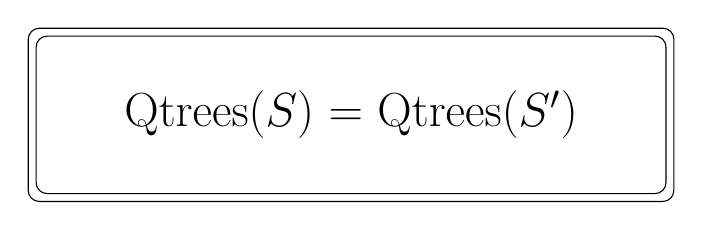
\begin{tikzpicture}
				\draw[rounded corners] (0, 0) rectangle (8, 2) {};
				\draw[rounded corners] (-.1, -.1) rectangle (8.1, 2.1) {};
				\node[] at(4,1) {\LARGE Qtrees($S$) = Qtrees($S'$)};
		\end{tikzpicture}}
		\caption[]{What a more ``intuitive'' version of \textsc{Q-Non-Redundancy} could have been ($S'$ refers to some simplification of $S$).}\label{fig4:redundancy-intuitive-extension}
	\end{subfigure}\hfill
	\begin{subfigure}[b]{.65\linewidth}
		\centering
		\scalebox{.7}{
			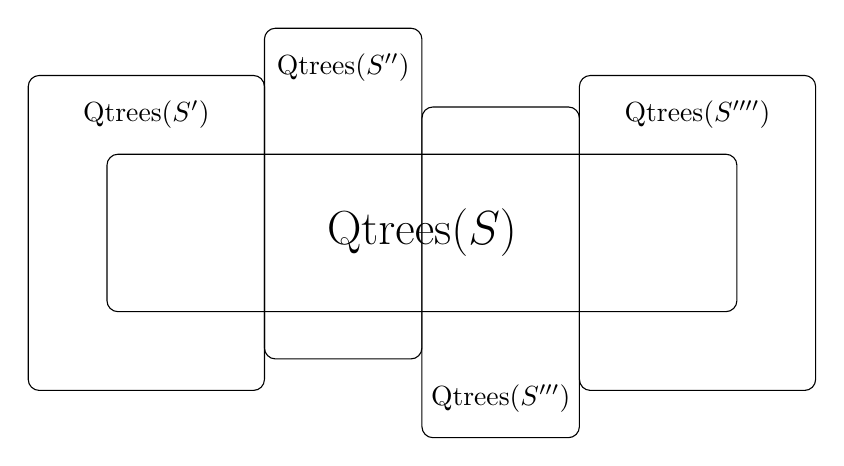
\begin{tikzpicture}
				\draw[rounded corners] (0, 0) rectangle (8, 2) {};
				\draw[rounded corners] (-1, -1) rectangle (2, 3) {};
				\draw[rounded corners] (6, -1) rectangle (9, 3) {};
				\draw[rounded corners] (4, -1.6) rectangle (6, 2.6) {};
				\draw[rounded corners] (2, -.6) rectangle (4, 3.6) {};
				\node[] at(.5,2.5) {Qtrees($S'$)};
				\node[] at(3,3.1) {Qtrees($S''$)};
				\node[] at(5,-1.1) {Qtrees($S'''$)};
				\node[] at(7.5,2.5) {Qtrees($S''''$)};
				\node[] at(4,1) {\LARGE Qtrees($S$)};
		\end{tikzpicture}}
		\caption[]{What it takes for $S$ to be \textsc{Q-Redundant} ($S'$, $S''$, $S'''$, and $S''''$ refer to simplifications of $S$).}\label{fig4:Q-Non-Redundancy}
	\end{subfigure}
	\caption[]{Comparing \textsc{Q-Non-Redundancy} to a more ``intuitive'' extension of \textsc{Manner} to the QuD domain.}
\end{figure}

Our definition of \textsc{Q-Non-Redundancy} also leaves space for other Qtree well-formedness constraints to contribute to a sentence's oddness. For instance a sentence $S$ may be deemed odd because \textit{some} Qtrees compatible with $S$ can be identified with \textit{some} Qtree generated by \textit{some} simplification of $S$ (violating \textsc{Q-Non-Redundancy}), and the other Qtrees compatible with $S$ are ruled-out \textsc{Empty Labeling}, or any other relevant constraint.\footnote{Chapter \ref{chap:hurford-sentence} will introduce another such constraint, \textsc{Q-Relevance}, which will enter the mix when evaluating sentence oddness.} This mixed-oddness profile is schematized in Figure \ref{fig4:Q-Non-Redundancy-relevance}.

\begin{figure}[H]
	\centering
	\scalebox{.7}{
		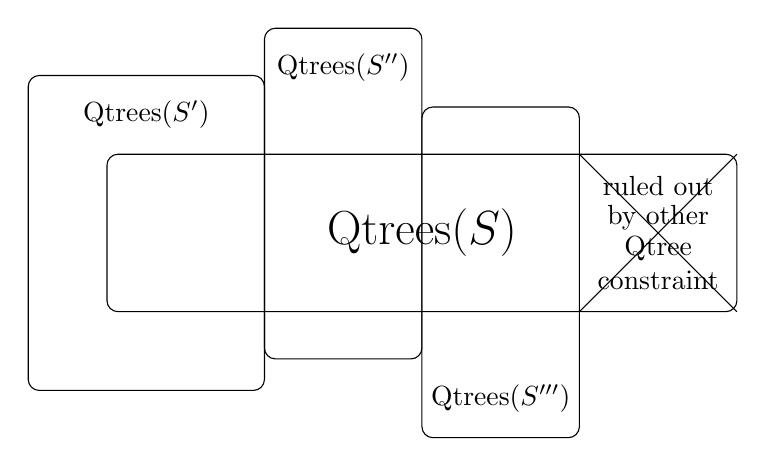
\begin{tikzpicture}
			\draw[rounded corners] (0, 0) rectangle (8, 2) {};
			\draw[rounded corners] (-1, -1) rectangle (2, 3) {};
			\draw[rounded corners] (4, -1.6) rectangle (6, 2.6) {};
			\draw[rounded corners] (2, -.6) rectangle (4, 3.6) {};
			\draw[-] (6,0) -- (8,2);
			\draw[-] (6,2) -- (8,0);
			\node[] at(.5,2.5) {Qtrees($S'$)};
			\node[] at(3,3.1) {Qtrees($S''$)};
			\node[] at(5,-1.1) {Qtrees($S'''$)};
			\node[] at(4,1) {\LARGE Qtrees($S$)};
			\node[] at(7,1.6) {{ruled out}};
			\node[] at(7,1.2) {{by other}};
			\node[] at(7,.8) {{Qtree}};
			\node[] at(7,.4) {{constraint}};
	\end{tikzpicture}}
	\caption[]{What it means for $S$ to be odd partly due to \textsc{Q-Non-Redundancy}, partly due to other Qtree well-formedness constraints, e.g. \textsc{Empty Flagging}.}\label{fig4:Q-Non-Redundancy-relevance}
\end{figure}



If \textsc{Q-Non-Redundancy} at the sentential level is not an intuitive extension of \textsc{Manner}, \textsc{Q-Non-Redundancy} defined on LF-Qtree pairs (see \ref{ex4:Q-Non-Redundancy}), is. To see this, one must define the simplification of a LF-Qtree \textit{pair} $(S, T)$, where $T$ is a Qtree evoked by $S$, as a pair ($S'$, $T'$) where $S'$ is a formal simplification of $S$ in the sense of (\ref{ex4:formal-simplification}), and $T'$ is a Qtree evoked by $S'$. Additionally, one must define equivalence between LF-Qtree pairs as equivalence between their Qtree-component. This yields a definition of \textsc{Q-Relevance}-as-\textsc{Manner}, given in (\ref{ex4:Q-Non-Redundancy-as-brevity}) that is set as a two-dimensional optimization problem on both LFs (which calibrate conciseness, and, indirectly, informativeness) and Qtrees (which calibrate informativeness).

\begin{exe}
	\ex 
	\begin{xlist}
		\ex \textit{LF-Qtree pair.} $(S, T)$ is a well-formed LF-Qtree pair iff $S$ evokes $T$.
		\ex \textbf{\textsc{Q-Redundancy}{\textit{ as} \textsc{Manner}}. If $(S, T)$ and ($S'$, $T'$) are two LF-Qtree pairs that are equivalent to each other, then the most concise of the two should be preferred.}
		\ex {\textit{Conciseness of a LF-Qtree pair.} If $(S, T)$ and ($S'$, $T'$) are two LF-Qtree pairs, ($S'$, $T'$) is more concise than $(S, T)$ iff $S'$ is a formal simplification of $S$ as per (\ref{ex4:structural-complexity}).}
		\ex {\textit{Equivalence between LF-Qtree pairs.} If $(S, T)$ and ($S'$, $T'$) are two LF-Qtree pairs, ($S'$, $T'$) is equivalent to $(S, T)$ iff $T = T'$.\footnote{This is simplified for the purposes of this paper: equality could be replaced by any more elaborate relation between Qtrees; see footnote \ref{fn:equivalence}, and Chapter \ref{chap:hurford-disj}.}}
	\end{xlist}\label{ex4:Q-Non-Redundancy-as-brevity}
\end{exe}

Now that we clarified how \textsc{Q-Non-Redundancy} can be seen as a proper extension of earlier pragmatic principles to the domain of LF-Qtree pairs, we discuss the effect of disjunct ordering on the felicitous (\ref{ex4:pv(nptq)-repeated}), as well as a few more interesting cases derived from the sentences in (\ref{ex4:target-sentences}).

\section{Exploring elaborations of the target sentences}\label{sec4:exploration}
\subsection{Effect of disjunct ordering in the felicitous case}\label{sec:ordering}

First, let us briefly come back to the pair (\ref{ex4:(nptq)vp})-(\ref{ex4:pv(nptq)}), repeated in (\ref{ex4:(nptq)vp-commut}). The two sentences in (\ref{ex4:(nptq)vp-commut}) only differ in the ordering of their disjuncts. At this point, we predict both to escape \textsc{Q-Non-Redundancy}, and more generally oddness. This, again, is because the introduction of $p$ as a disjunct makes it at-issue, while it would be ``neglected'' if the sentence were simplified into its conditional disjunct. (\ref{ex4:(nptq)vp-repeated}) however, sounds worse than (\ref{ex4:pv(nptq)-repeated-2}), and even more so if the conditional disjunct did not feature inversion.

\begin{exe}
	\ex \label{ex4:(nptq)vp-commut}
	\begin{xlist}
		\ex[] {Either Jo is at SuB or if he is not at SuB then he is in Cambridge.\\ $\p \vee (\neg \p \rightarrow \q)$}\label{ex4:pv(nptq)-repeated-2}
		\ex[?] {Either Jo is in Cambridge if not at SuB, or he is at SuB.\\ $(\neg \p \rightarrow \q) \vee \p$}\label{ex4:(nptq)vp-repeated}
	\end{xlist}
\end{exe}

We suggest this contrast is caused by an independent, incremental constraint targeting Qtree derivations. As observed in Section \ref{sec:rule-in}, (\ref{ex4:pv(nptq)-repeated-2}) is compatible with two well-formed Qtrees, repeated in Figure \ref{fig4:qtrees-pv(nptq)-non-redundant}. Figures \ref{fig4:qtrees-p-1st-disj} and \ref{fig4:qtrees-nptq-2nd-disj} summarize the ``ingredients'' used to derive these two disjunctive Qtrees: a Qtree for $p$, and two possible Qtrees for $\neg p \rightarrow q$.

\begin{figure}[H]
	\centering
	\begin{subfigure}[b]{.45\linewidth}
		\centering
		\scalebox{1}{
			\begin{forest}
				[CS [{\fbox{$\p$}}][{$\neg \p$} [\fbox{$\q$}][$\neg \q \cap \neg \p$]]]
			\end{forest}
		}
		\caption[]{Tree \ref{fig4:qtree-p-polar} $\vee$ Tree \ref{fig4:qtree-nptq-polar-polar}.}\label{fig4:qtree-pv(nptq)-polar-polar-repeated}
	\end{subfigure}\hfill
	\begin{subfigure}[b]{.45\linewidth}
		\centering
		\scalebox{1}{
			\begin{forest}
				[CS [{\fbox{$\p$}}][{$\neg \p$} [\fbox{$\q$}][$\r$][...]]]
			\end{forest}
		}
		\caption[]{Tree\ref{fig4:qtree-p-polar} $\vee$ Tree  \ref{fig4:qtree-nptq-polar-wh}.}\label{fig4:qtree-pv(nptq)-polar-wh-repeated}
	\end{subfigure}
	\caption[]{Non \textsc{Q-Redundant} Qtrees for (\ref{ex4:pv(nptq)-repeated})/(\ref{ex4:pv(nptq)-repeated-2}) $= \p \vee (\neg \p \rightarrow \q)$.}\label{fig4:qtrees-pv(nptq)-non-redundant}
\end{figure}

\begin{figure}[H]\setlength{\fboxsep}{2pt}
	\centering
		\scalebox{1}{
			\begin{forest}
				[CS [\fbox{\p}] [$\neg \p$]]
			\end{forest}
		}
	\caption[]{Qtree for $\p =$ \textit{Jo is at SuB} (first disjunct of (\ref{ex4:pv(nptq)-repeated})/(\ref{ex4:pv(nptq)-repeated-2})), used to derive the Qtrees in Figure \ref{fig4:qtrees-pv(nptq)-non-redundant}.}
	\label{fig4:qtrees-p-1st-disj}
\end{figure}


\begin{figure}[H]\setlength{\fboxsep}{2pt}
	\centering
	\begin{subfigure}[b]{.45\linewidth}
		\centering
		\scalebox{1}{
			\begin{forest}
				[CS [{$\p$}][{$\neg \p$} [\textcolor{red}{\fbox{$\q$}}][$\neg \q \cap \neg \p$]]]
			\end{forest}
		}
		\caption[]{Tree \ref{fig4:qtree-np-polar} $\rightarrow$ Tree \ref{fig4:qtree-q-polar}.}
	\end{subfigure}\hfill
	\begin{subfigure}[b]{.45\linewidth}
		\centering
		\scalebox{1}{
			\begin{forest}
				[CS [{$\p$}][{$\neg \p$} [\textcolor{red}{\fbox{$\q$}}][$\r$][...]]]
			\end{forest}
		}
		\caption[]{Tree \ref{fig4:qtree-np-polar} $\rightarrow$ Tree \ref{fig4:qtree-q-wh}.}
	\end{subfigure}
	\caption[]{Qtrees for $\neg \p \rightarrow\q =$ \textit{If Jo is not at SuB then he is in Cambridge} (second disjunct of (\ref{ex4:pv(nptq)-repeated})/(\ref{ex4:pv(nptq)-repeated-2})), used to derive the Qtrees in Figure \ref{fig4:qtrees-pv(nptq)-non-redundant}.}
	\label{fig4:qtrees-nptq-2nd-disj}
\end{figure}

We observe that the Qtree in Figure \ref{fig4:qtrees-p-1st-disj}, which is evoked by $p$ and corresponds to the first disjunct of (\ref{ex4:pv(nptq)-repeated-2}), is structurally contained in the Qtrees in Figure \ref{fig4:qtrees-nptq-2nd-disj}, which are evoked by $\neg p \rightarrow q$ and correspond to the second disjunct of (\ref{ex4:pv(nptq)-repeated-2}). In other words, (\ref{ex4:pv(nptq)-repeated-2})'s first disjunct evokes a Qtree that is coarser-grained (i.e. less specific) than the Qtrees evoked by (\ref{ex4:pv(nptq)-repeated-2})'s second disjunct. The opposite holds for (\ref{ex4:(nptq)vp-repeated}). In other words, the disjunction in (\ref{ex4:pv(nptq)-repeated-2}) takes two Qtrees of increasing specificity as input (from left to right), while the disjunction in (\ref{ex4:(nptq)vp-repeated}) takes two Qtrees of decreasing specificity. And it is reasonable to think that the latter order should be preferred. This is supported by the sequences of questions in (\ref{ex4:q-ordering}): it appears more natural to ask a less specific question (e.g., about countries), before a more specific one (e.g., about cities), than the other way around.\footnote{Similar considerations will ground our definition of \textsc{Q-Relevance} in Chapter \ref{chap:hurford-sentences}, in the context of Hurford Conditionals. \textsc{Q-Relevance} will yield slightly more subtle predictions than (\ref{ex4:incr-containment}).} The latter ordering in fact seems to suggest that the more specific question would not allow to infer the exact answer to the less specific one.

\begin{exe}
	\ex \label{ex4:q-ordering}
	\begin{xlist}
		\ex[] {In which country does Jo live? And in which city?}
		\ex[?] {In which city does Jo live? And in which country?}
	\end{xlist}
\end{exe} 

Assuming that the country-level questions in (\ref{ex4:q-ordering}) are structurally contained in the city-level questions (as argued in Chapter \ref{chap:accommodating-quds}), we derive the following generalization covering both (\ref{ex4:(nptq)vp-commut}) and (\ref{ex4:q-ordering}).\footnote{(\ref{ex4:q-ordering}) may seem reminiscent of Hurford Disjunctions \citep{Hurford1974}. Chapter \ref{chap:hurford-disj} will predict Hurford Disjunctions to be bad in \textit{both} orders due to an updated version of \textsc{Q-Non-Redundancy}, i.e., \textit{independently} of the constraint in (\ref{ex4:incr-containment}).}

\begin{exe}
	\ex {\textsc{\textbf{Incremental Qtree Containment}.} Let $X$ and $Y$ be LFs, and $\circ$ be a binary operator. If $X \circ Y$ and $Y \circ X$ have same meaning and same evoked Qtrees, and if $\forall T \in Qtrees(X \circ Y)$, $T$ is obtained from $T' \in Qtrees(X)$ and $T'' \in Qtrees(Y)$ with $T' \subset T''$, then $X \circ Y$ should be preferred over $Y \circ X$.}\label{ex4:incr-containment}
\end{exe}



\subsection{Double or-to-if}\label{sec4:double-or-if}

Before wrapping this Chapter, let us briefly discuss more complex variants of (\ref{ex4:double-disjunctions}), derived \textit{via} two applications of the \textit{or-to-if} tautology. (\ref{ex4:nptnptq}) sounds clearly redundant, while (\ref{ex4:nptnqtp}) and  (\ref{ex4:nptnqtp}) somehow feel contradictory. (\ref{ex4:nnqtptp}) and (\ref{ex4:nnqtptp}) appear very tough to make sense of. 
\begin{exe}
	\ex\label{ex4:double-or-if}
	\begin{xlist}
		\ex[\#] {If Jo isn't at SuB then, if he isn't at SuB then he is in Cambridge.\\ $\neg \p \rightarrow (\neg \p \rightarrow \q)$}\label{ex4:nptnptq}
		\ex[\#] {If Jo isn't at SuB then, if he isn't in Cambridge then he is at SuB.\\ $\neg \p \rightarrow (\neg \q \rightarrow \p)$}\label{ex4:nptnqtp}
		\ex[??] {If it's not that Jo is in Cambridge if not at SuB, then he isn't at SuB.\\ $\neg (\neg \p \rightarrow \q) \rightarrow \p$}\label{ex4:nnptqtp}
		\ex[\#] {If it's not that Jo is at SuB if not in Cambridge, then Jo is at SuB.\\ $\neg (\neg \q \rightarrow \p) \rightarrow \p$}\label{ex4:nnqtptp}
	\end{xlist}
\end{exe}





The model laid out in this paper predicts all the sentences in (\ref{ex4:double-or-if}) to be odd, for different reasons. (\ref{ex4:nptnptq}) turns out \textsc{Q-Redundant}, because all the Qtrees it gives rise to are the same as the ones generated by its consequent $\neg p \rightarrow q$ (see Figure \ref{fig4:qtrees-nptq}). Both (\ref{ex4:nptnqtp}) and (\ref{ex4:nnqtptp}) generate Qtrees that invariably display \textsc{Empty Flagging}, see Figures \ref{fig4:qtrees-npt(nqtp)} and \ref{fig4:qtrees-n(nqtp)tp}. In both cases, this can be traced back to the fact that the ``restrictor'' nodes in which the consequent Qtree is ``plugged'', are sets of $\neg p$-worlds, and $p$ is precisely what the consequent Qtree would have contributed as verifying node.


\begin{figure}[H]
	\centering
	\begin{subfigure}[b]{.45\linewidth}
		\centering
		\scalebox{1}{
			\begin{forest}
				[CS[\p][$\neg\p$[\q][$\neg\q\cap\neg\p$]]]
			\end{forest}
		}
		\caption[]{Tree \ref{fig4:qtree-np-polar} $\rightarrow$ Tree \ref{fig4:qtree-nqtp-polar-polar}.}
	\end{subfigure}
	\hfill
	\begin{subfigure}[b]{.45\linewidth}
		\centering
		\scalebox{1}{
			\begin{forest}
				[CS[\p][$\neg\p$[\q][$\neg\q\cap\neg\p$[\r][...]]]]
			\end{forest}
		}
		\caption[]{Tree \ref{fig4:qtree-np-polar} $\rightarrow$ Tree \ref{fig4:qtree-nqtp-polar-wh}.}
	\end{subfigure}
\end{figure}
\begin{figure}[H]
	\centering
	\ContinuedFloat
	\begin{subfigure}[b]{.45\linewidth}
		\centering
		\scalebox{1}{
			\begin{forest}
				[CS[\p][$\neg\p$[\q][\r][...]]]
			\end{forest}
		}
		\caption[]{Tree \ref{fig4:qtree-np-polar} $\rightarrow$ Tree \ref{fig4:qtree-nqtp-wh}.}
	\end{subfigure}
	\hfill
	\begin{subfigure}[b]{.45\linewidth}
		\centering
		\scalebox{1}{
			\begin{forest}
				[CS[\p][\q][\r][...]]
			\end{forest}
		}
		\caption[]{Tree \ref{fig4:qtree-np-wh} $\rightarrow$ Tree \ref{fig4:qtree-nqtp-polar-polar} / \ref{fig4:qtree-nqtp-polar-wh} /  \ref{fig4:qtree-nqtp-wh}.}
	\end{subfigure}
	\caption[]{Qtrees for \#(\ref{ex4:nptnqtp}) = $\neg\p \rightarrow(\neg\q \rightarrow\p)$. \textbf{Odd due to \textsc{Empty Labeling}}.}\label{fig4:qtrees-npt(nqtp)}
\end{figure}


\begin{figure}[H]
	\centering
	\begin{subfigure}[b]{.45\linewidth}
		\centering
		\scalebox{1}{
			\begin{forest}
				[CS[\q][$\neg\q$[\p][$\neg\p\cap\neg\q$[\r][...]]]]
			\end{forest}
		}
		\caption[]{$\neg$(Tree \ref{fig4:qtree-nqtp-polar-polar}) $\rightarrow$ Tree \ref{fig4:qtree-p-wh}.\\ \textbf{\textsc{Empty Labeling}}.}
	\end{subfigure}
	\hfill
	\begin{subfigure}[b]{.45\linewidth}
		\centering
		\scalebox{1}{
			\begin{forest}
				[CS[\q][$\neg\q$[\p][$\neg\p\cap\neg\q$]]]
			\end{forest}
		}
		\caption[]{$\neg$(Tree \ref{fig4:qtree-nqtp-polar-polar}) $\rightarrow$ Tree \ref{fig4:qtree-p-polar}.\\ \textbf{\textsc{Empty Labeling}}.}
	\end{subfigure}
\end{figure}
\begin{figure}[H]
\centering
\ContinuedFloat	
	\begin{subfigure}[b]{.45\linewidth}
		\centering
		\scalebox{1}{
			\begin{forest}
				[CS[\q][$\neg\q$[\p][\r][...]]]
			\end{forest}
		}
		\caption[]{$\neg$(Tree \ref{fig4:qtree-nqtp-polar-wh}) $\rightarrow$ Tree \ref{fig4:qtree-p-polar} / \ref{fig4:qtree-p-wh}.\\ \textbf{\textsc{Empty Labeling}}.}
	\end{subfigure}
	\hfill
	\begin{subfigure}[b]{.45\linewidth}
		\centering
		\scalebox{1}{
			\begin{forest}
				[CS[\p][\q][\r][...]]
			\end{forest}
		}
		\caption[]{$\neg$(Tree \ref{fig4:qtree-nqtp-wh}) $\rightarrow$ Tree \ref{fig4:qtree-p-polar} / \ref{fig4:qtree-p-wh}.\\ \textbf{\textsc{Empty Labeling}}.}
	\end{subfigure}
	\caption[]{Qtrees for \#(\ref{ex4:nnqtptp}) = $\neg (\neg \q \rightarrow \p) \rightarrow \p$. \textbf{Odd due to \textsc{Empty Labeling}}.}\label{fig4:qtrees-n(nqtp)tp}
\end{figure}

Lastly, (\ref{ex4:nnptqtp}) represents a mixed case of oddness: most of the Qtrees it evokes display \textsc{Empty Flagging}, and one tree turns out \textsc{Q-Redundant} due to the $p$-simplification of the sentence. This is further detailed in Figure \ref{fig4:qtrees-n(nptq)tp}. 
\begin{figure}[H]
	\centering
	\begin{subfigure}[b]{.45\linewidth}
		\centering
		\scalebox{1}{
			\begin{forest}
				[CS[\p][$\neg\p$[\q][$\neg\p\cap\neg\q$]]]
			\end{forest}
		}
		\caption[]{$\neg$(Tree \ref{fig4:qtree-nptq-polar-polar}) $\rightarrow$ Tree \ref{fig4:qtree-p-polar}.\\ \textbf{\textsc{Empty Labeling}}.}
	\end{subfigure}
	\hfill
	\begin{subfigure}[b]{.45\linewidth}
		\centering
		\scalebox{1}{
			\begin{forest}
				[CS[\p][$\neg\p$[\q][$\neg\p\cap\neg\q$[\r][...]]]]
			\end{forest}
		}
		\caption[]{$\neg$(Tree \ref{fig4:qtree-nptq-polar-polar}) $\rightarrow$ Tree \ref{fig4:qtree-p-wh}.\\ \textbf{\textsc{Empty Labeling}}.}
	\end{subfigure}
\end{figure}
\begin{figure}[H]
\centering
\ContinuedFloat	
	\begin{subfigure}[b]{.45\linewidth}
		\centering
		\scalebox{1}{
			\begin{forest}
				[CS[\p][$\neg\p$[\q][\r][...]]]
			\end{forest}
		}
		\caption[]{$\neg$(Tree \ref{fig4:qtree-nptq-polar-wh}) $\rightarrow$ Tree \ref{fig4:qtree-p-polar} / \ref{fig4:qtree-p-wh}.\\ \textbf{\textsc{Empty Labeling}}.}
	\end{subfigure}
	\hfill
	\begin{subfigure}[b]{.45\linewidth}
		\centering
		\scalebox{1}{
			\begin{forest}
				[CS[\fbox{\p}][\q][\r][...]]
			\end{forest}
		}
		\caption[]{$\neg$(Tree \ref{fig4:qtree-nptq-wh}) $\rightarrow$ Tree \ref{fig4:qtree-p-polar} / \ref{fig4:qtree-p-wh}.\\ \textbf{Same as Figure \ref{fig4:qtree-p-wh}}.}\label{fig4:qtree-n(nptq)tp-wh}
	\end{subfigure}
	\caption[]{Qtrees for ??(\ref{ex4:nnptqtp}) = $\neg (\neg \p \rightarrow \q) \rightarrow \p$. \textbf{Odd for mixed reasons (\textsc{Empty Labeling}/\textsc{Q-Non-Redundancy})}.}\label{fig4:qtrees-n(nptq)tp}
\end{figure}

It is worth mentioning that some of the Qtrees in Figure \ref{fig4:qtrees-n(nptq)tp}, were computed from Qtrees that \textit{themselves} were not complying with Qtree well-formedness constraints. For instance, the Qtree in Figure \ref{fig4:qtree-n(nptq)tp-wh} (which turns out \textsc{Q-Redundant} given (\ref{ex4:nnptqtp})), is derived using the Qtree in Figure \ref{fig4:qtree-nptq-wh}, which is itself \textsc{Q-Redundant} given $\neg q\rightarrow p$. Maybe this derivation should have been blocked altogether, in virtue of one of its inputs being \textsc{Q-Redundant}. More generally, this raises the question whether \textsc{Non-Q-Redundancy} should apply globally (\textit{à la} \textsc{Global Redundancy}), i.e. once all the possible Qtrees for a given sentence are derived, or, locally (\textit{à la} \textsc{Local Redundancy}), i.e. each time a Qtree is compositionally derived from input Qtree(s). We leave this question for future work.
%Jo had dessert or cheese and dessert
%if Jo did not have dessert he had cheese and dessert
%if Jo did not have cheese and dessert he had dessert



\section{Conclusion and outlook}\label{sec4:conclusion}
In this Chapter, we presented novel data based on logical variants of $p \vee p \vee q$, that appeared challenging to account for while retaining classic results on other families of odd sentences, in particular Hurford Disjunctions and Conditionals \citep{Hurford1974, Mandelkern2018}. In particular, these data appeared problematic for \citeauthor{Kalomoiros2024}'s recent account, otherwise characterized by a wide empirical coverage, including the very challenging Hurford Conditionals.\\

This Chapter then proposed an account of the problematic paradigm in the QuD-framework, based on two core ideas introduced in Chapter \ref{chap:accommodating-quds}, namely, that sentences have to be good answer to good questions \citep{Katzir2015}, and that disjunctions and conditionals evoke distinct kinds of questions (Qtrees). Beyond these two insights, we devised a novel implementation of \textsc{Non-Redundancy}, which was made sensitive to how sentences ``package'' information \textit{via} their Qtree. The next two Chapters extend this framework to capture Hurford Disjunctions and Conditionals \citep{Hurford1974,Mandelkern2018} -- leading us to update \textsc{Q-Non-Redundancy}, and to introduce yet another Qtree well-formedness constraint, in the form of \textsc{Q-Relevance}. More broadly, this approach suggests that oddness may come in different ``flavors'' and that sentences may be odd due to a conspiration of these various factors.\\

A WORD ON THE CONJUNCTIVE ALTERNATIVE FROM MAYR AND ROMOLI??
%More generally, this predicts ``connectivity effects'' in disjunctions-of-conditionals, in that the antecedents and consequents respectively have to address similar QuDs; and no such effect in conditionals-of-disjunctions, in that disjuncts coming from the antecedent and consequent may be inquisitively unrelated.
%ido had dessert or cheese and dessert
%if ido did not have dessert he had cheese and dessert
%if ido did not have cheese and dessert he had dessert







